%% monografia.tex, fabiokepler, jeancheiran
%% Copyright 2012-2018 by UNIPAMPA LaTeX group at https://bitbucket.org/unipampaalegrete/monografias-cc-es-repo/
%%
%% This work may be distributed and/or modified under the conditions of the LaTeX Project Public
%% License, either version 1.3 of this license or (at your option) any later version.
%% The latest version of this license is in
%%   http://www.latex-project.org/lppl.txt
%% and version 1.3 or later is part of all distributions of LaTeX version 2005/12/01 or later.
%%
%% Based on the example file abtex2-modelo-trabalho-academico.tex of the abntex2 package
%% (http://abntex2.googlecode.com/) and on the ppgccufmg 1.45beta2 class
%% (http://vilarneto.com/ppgccufmg,
%% http://www.dcc.ufmg.br/pos/alunos/modelodisstese.php
%% and http://www.dcc.ufmg.br/~mirella).
%%
%% Adapted for the Computer Science program at UNIPAMPA (http://www.unipampa.edu.br)
%% by Fabio Kepler (fabio@kepler.pro.br) and Jean Cheiran (jeancheiran@unipampa.edu.br).
%%
%% Version 2.5 - 2018/08
%% Version 2.4 - 2017/05
%% Version 2.3 - 2013/03

% +++++++++++++++++++++++++++++++++++++++++++++++++++++++++++++++++++++++++++++++++++++++++++++++++
% Este modelo utiliza o pacote abnTeX2. Veja como instalá-lo em seu ambiente em
% http://abntex2.googlecode.com/.
% -------------------------------------------------------------------------------------------------
% abnTeX2: Modelo de Trabalho Acadêmico (tese de doutorado, dissertação de
% mestrado e trabalhos monográficos em geral) em conformidade com
% ABNT NBR 14724:2011: Informação e documentação - Trabalhos acadêmicos -
% Apresentação
% -------------------------------------------------------------------------------------------------
% Normas institucionais utilizadas:
% http://porteiras.r.unipampa.edu.br/portais/sisbi/programa-de-capacitacao/
% +++++++++++++++++++++++++++++++++++++++++++++++++++++++++++++++++++++++++++++++++++++++++++++++++

\documentclass[12pt,openright,twoside,a4paper,chapter=TITLE]{abntex2}    % frente e verso
%\documentclass[12pt,oneside,a4paper]{abntex2}            % apenas frente

% +++++++++++++++++++++++++++++++++++++++++++++++++++++++++++++++++++++++++++++++++++++++++++++++++
% PACOTES
% -------------------------------------------------------------------------------------------------
% Pacotes fundamentais
\usepackage{cmap}           % Mapeamento de caracteres especiais no PDF
\usepackage{lmodern}        % Usa fonte Latin Modern
\usepackage[T1]{fontenc}    % Seleção de codificação de fonte
\usepackage[utf8]{inputenc} % Codificação do arquivo (conversão automática dos acentos)
\usepackage[brazil]{babel}  % Idioma para hifenização e tradução de vários elementos
\usepackage{makeidx}        % Criação de índice
\usepackage{hyperref}       % Formatação do índice
\usepackage{lastpage}       % Usado pela Ficha catalográfica
\usepackage{indentfirst}    % Indenta o primeiro parágrafo de cada seção
\usepackage[usenames,dvipsnames]{xcolor}  % Controle das cores (com nomes)
\usepackage{graphicx}       % Inclusão de gráficos
\usepackage{booktabs}       % Formatação de tabelas
% -------------------------------------------------------------------------------------------------
% Para citações
\usepackage[brazilian,hyperpageref]{backref} % Páginas com as citações na bibliografia
\usepackage[alf,abnt-emphasize=bf]{abntex2cite} % Citações padrão ABNT (alfanumérico)
% -------------------------------------------------------------------------------------------------
% Pacotes opcionais
\usepackage{nomencl}        % Para criar uma lista de símbolos
\usepackage{acro}           % Para usar acrônimos e abreviaturas
\usepackage{tikz}           % Para fazer figuras, diagramas e gráficos integrados e elegantes
\usepackage{pgfplots}       % Usa o pacote tikz para fazer gráficos muito melhores que os do Excel
\usepackage{pgfplotstable}  % Para gerar tabelas automaticamente a partir de arquivos com dados
\usepackage{filecontents}   % Para colocar o conteúdo de um arquivo dentro de um arquivo tex
\usepackage{todonotes}      % Para criar anotações durante o desenvolvimento do texto
%\usepackage{multirow}       % Permite fazer tabelas com múltiplas linhas
%\let\newfloat=\undefined    % Workaround para usar o pacote algorithm
%\usepackage{algorithm}      % Para escrever algoritmos
%\usepackage{clrscode}       % Para escrever algoritmos
%\usepackage{clrscode3e}     % Para escrever algoritmos; mais simples que os pacotes acima
\usepackage{pdfpages}        % Para incluir a folha de aprovação assinada em PDF
\usepackage{paralist}       % Listas in-line
% -------------------------------------------------------------------------------------------------
% Configurações de pacotes
% -------------------------------------------------------------------------------------------------
% \addto\captionsbrazil{
%   \renewcommand{\listfigurename}{List of figures}
% }
% -------------------------------------------------------------------------------------------------
\addto\captionsenglish{% ingles
  %% adjusts names from abnTeX2
  \renewcommand{\folhaderostoname}{Title page}
  \renewcommand{\epigraphname}{Epigraph}
  \renewcommand{\dedicatorianame}{Dedication}
  \renewcommand{\errataname}{Errata sheet}
  \renewcommand{\agradecimentosname}{Acknowledgements}
  \renewcommand{\anexoname}{ANNEX}
  \renewcommand{\anexosname}{Annex}
  \renewcommand{\apendicename}{APPENDIX}
  \renewcommand{\apendicesname}{Appendix}
  \renewcommand{\orientadorname}{Supervisor:}
  \renewcommand{\coorientadorname}{Co-supervisor:}
  \renewcommand{\folhadeaprovacaoname}{Approval}
  \renewcommand{\resumoname}{Resumo} 
  \renewcommand{\listadesiglasname}{List of abbreviations and acronyms}
  \renewcommand{\listadesimbolosname}{List of symbols}
  \renewcommand{\fontename}{Source}
  \renewcommand{\notaname}{Note}
   %% adjusts names used by \autoref
  \renewcommand{\pageautorefname}{page}
  \renewcommand{\sectionautorefname}{section}
  \renewcommand{\subsectionautorefname}{subsection}
  \renewcommand{\subsubsectionautorefname}{subsubsection}
  \renewcommand{\paragraphautorefname}{subsubsubsection}
  \renewcommand{\englishbibname}{Bibliography}
  \renewcommand{\englishindexname}{Index}
  \renewcommand{\englishlistfigurename}{List of figures}
  \renewcommand{\englishfigurename}{Figure}
  \renewcommand{\englishlisttablename}{List of tables}
  \renewcommand{\englishtablename}{Table}
  \renewcommand{\englishcontentsname}{List of contents}
   \renewcommand{\imprimirtipotrabalho}{Term Paper }
}
% Configurações do pacote backref
% Usado sem a opção hyperpageref de backref
\renewcommand{\backrefpagesname}{Cited in page(s):~}
% Texto padrão antes do número das páginas
\renewcommand{\backref}{}
% Define os textos da citação
\renewcommand*{\backrefalt}[4]{
    \ifcase #1 %
        No text citation.%
    \or
        Cited in page #2.%
    \else
        Cited #1 times on pages #2.%
    \fi}%
% -------------------------------------------------------------------------------------------------
% Configurações de aparência do PDF final
%\definecolor{blue}{RGB}{41,5,195}
% \definecolor{webgreen}{rgb}{0,.5,0}
% Metainformações do PDF e cores dos links
\hypersetup{
  portuguese,
  %backref=true,
  %pagebackref=true,
  %bookmarks=true,             % show bookmarks bar?
  %bookmarksnumbered=true,
  bookmarksdepth=4,
  pdftitle={\@title},
  pdfauthor={\@author},
  pdfsubject={\imprimirpreambulo},
  pdfkeywords={UNIPAMPA}{Computação}{UNIPAMPA}{abntex}{TCC},
  %pdfproducer={LaTeX with abnTeX2},     % producer of the document
  pdfcreator={\@author},
  colorlinks=true,           % false: boxed links; true: colored links
  linkcolor=black,            % color of internal links
  citecolor=black,            % color of links to bibliography
  filecolor=black,         % color of file links
  urlcolor=black
}
%   linktocpage,
%   colorlinks,
%   citecolor=webgreen,
%   urlcolor=Maroon,
%   linkcolor=RoyalBlue,
%   filecolor=black,
% -------------------------------------------------------------------------------------------------
% Espaçamentos entre linhas e parágrafos
% O tamanho do parágrafo é dado por
\setlength{\parindent}{1.3cm}
% Controle do espaçamento entre um parágrafo e outro
\setlength{\parskip}{0.2cm} % tente também \onelineskip
% Controles do espaçamento entre linhas
%\OnehalfSpacing       % espaçamento um e meio (padrão);
%\DoubleSpacing        % espaçamento duplo
%\SingleSpacing        % espaçamento simples
% -------------------------------------------------------------------------------------------------
% Para o pacote de acrônimos
\acsetup{make-links} %first-style=short}
% -------------------------------------------------------------------------------------------------
% Para o pacote tikz, pgfplots e pgfplotstable
\usetikzlibrary{arrows,chains,matrix,positioning,decorations.pathreplacing,calc}
% -------------------------------------------------------------------------------------------------
% Para poder usar subfiguras e subtabelas
\newsubfloat{figure}
\newsubfloat{table}
\providecommand*{\subfigureautorefname}{\figureautorefname}
% +++++++++++++++++++++++++++++++++++++++++++++++++++++++++++++++++++++++++++++++++++++++++++++++++


% +++++++++++++++++++++++++++++++++++++++++++++++++++++++++++++++++++++++++++++++++++++++++++++++++
% Informações de dados para CAPA e FOLHA DE ROSTO
% -------------------------------------------------------------------------------------------------
\titulo{Extensionly - A tool for supporting the management of extracurricular projects and programs: Frontend}
\autor{Lucas Alexandre Fell}
\local{Alegrete}
\data{2022}
\orientador{Prof. PhD. Maicon Bernardino da Silveira}
% \coorientador{Prof. <titulação> Nome do Coorientador} % Se houver
\instituicao{Federal University of Pampa}
%\tipotrabalho{Projeto de Trabalho de Conclusão de Curso~} % Para TCC I
\tipotrabalho{Trabalho de Conclusão de Curso~} % Para TCC II
% O preambulo deve conter o tipo do trabalho, o objetivo, o nome da instituição e a área de concentração
\preambulo{\imprimirtipotrabalho presented in Software Engineering Graduation Course in the Federal University of Pampa as a partial requirement for
obtaining the title of Software Engineering
Bachelor}
% +++++++++++++++++++++++++++++++++++++++++++++++++++++++++++++++++++++++++++++++++++++++++++++++++

% -------------------------------------------------------------------------------------------------
% Compila o indice
\makeindex
% Compila a lista de abreviaturas e siglas
% Para funcionar, o seguinte comando deve ser executado:
% makeindex ARQUIVO_PRINCIPAL.nlo -s nomencl.ist -o ARQUIVO_PRINCIPAL.nls
\makenomenclature
% -------------------------------------------------------------------------------------------------

% -------------------------------------------------------------------------------------------------
% Abreviaturas 
\DeclareAcronym{fig}{
  short = Fig.,
  long  = Figura,
  tag = abreviaturas
}
% Acrônimos/Siglas
\DeclareAcronym{UNIPAMPA}{
  short = Unipampa,
  long  = Federal University of Pampa,
  tag = acronimos
}
\DeclareAcronym{OCA}{
  short = OCA,
  long  = Outreach Curriculum Activity,
  long-plural-form = Outreach Curriculum Activities,
  tag = acronimos
}
\DeclareAcronym{OA}{
  short = OA,
  long  = Outreach Activity,
  long-plural-form = Outreach Activities,
  tag = acronimos
}
\DeclareAcronym{PROEXT}{
  short = PROEXT,
  long  = Dean of Outreach and Culture,
  tag = acronimos
}
\DeclareAcronym{IT}{
  short = IT,
  long  = Information Technology,
  tag = acronimos
}
\DeclareAcronym{MVP}{
  short = MVP,
  long  = Minimum Viable Product,
  tag = acronimos
}
\DeclareAcronym{FORPROEX}{
  short = FORPROEX,
  long  = Forum of Pro-Rectors for Outreach of Brazilian Public Universities,
  tag = acronimos
}
\DeclareAcronym{HEI}{
  short = HEI,
  long  = Higher Education Institution,
  tag = acronimos
}
\DeclareAcronym{HECI}{
  short = HECI,
  long  = Higher Education Community Institution,
  tag = acronimos
}
\DeclareAcronym{SIGAA}{
  short = SIGAA,
  long  = Integrated Academic Activities Management System,
  tag = acronimos
}
\DeclareAcronym{ATE}{
  short = ATE,
  long  = Administrative Technician in Education,
  tag = acronimos
}
\DeclareAcronym{SGCE}{
  short = SGCE,
  long  = Electronic Certificate Management System,
  tag = acronimos
}
\DeclareAcronym{SIPPEE}{
  short = SIPPEE,
  long  = {Information System for Research, Teaching and Outreach Projects},
  tag = acronimos
}
\DeclareAcronym{NGO}{
  short = NGO,
  long  = Non-governmental organization,
  long-plural-form = Non-governmental organizations,
  tag = acronimos
}
\DeclareAcronym{CAEX}{
  short = CAEX,
  long  = Outreach Actions Control,
  tag = acronimos
}
\DeclareAcronym{MoSCoW}{
  short = MoSCoW,
  long  = {Must have, Should have, Could have and Will not have},
  tag = acronimos
}
\DeclareAcronym{API}{
  short = API,
  long  = {Application Programming Interface},
  tag = acronimos
}
\DeclareAcronym{ID}{
  short = ID,
  long  = {Identification},
  tag = acronimos
}
\DeclareAcronym{SAP}{
  short = SAP,
  long  = Academic Project System,
  tag = acronimos
}
\DeclareAcronym{SEI}{
  short = SEI,
  long  = Electronic Information System,
  tag = acronimos
}
\DeclareAcronym{FR}{
  short = FR,
  long  = Functional Requirement,
  tag = acronimos
}
% -------------------------------------------------------------------------------------------------
% Nomenclaturas/Símbolos
% \nomenclature{$A_i$}{Área do $i^{esimo}$ componente}
% \nomenclature{456}{Isto é um número}
% \nomenclature{123}{Isto é outro número}
% \nomenclature{$n$}{Tamanho da entrada}
% \nomenclature{$V$}{Vetor de elementos}
% \nomenclature{$\mathcal{T}$}{Conjunto de trabalhos de TCC}

% -------------------------------------------------------------------------------------------------
% Inclui alguns ajustes finos para que fique de acordo com o Manual de Normatização
% Pequenos consertos e ajustes para que fique de acordo com o Manual de Normatização 2011.

\setlength{\ABNTEXsignwidth}{12cm}

%% adjusts names from abnTeX2
% \renewcommand{\folhaderostoname}{Title page}
% \renewcommand{\epigraphname}{Epigraph}
% \renewcommand{\dedicatorianame}{Dedication}
% \renewcommand{\errataname}{Errata sheet}
% \renewcommand{\agradecimentosname}{Acknowledgements}
% \renewcommand{\anexoname}{ANNEX}
% \renewcommand{\anexosname}{Annex}
% \renewcommand{\apendicename}{APPENDIX}
% \renewcommand{\apendicesname}{Appendix}
% \renewcommand{\orientadorname}{Supervisor:}
% \renewcommand{\coorientadorname}{Co-supervisor:}
% \renewcommand{\folhadeaprovacaoname}{Approval}
% % \renewcommand{\resumoname}{Resumo
% % \renewcommand{\englishcontentsname}{Summary}
% % \renewcommand{\englishlistfigurename}{List of figures}
% % \renewcommand{\englishlisttablename}{List of tables}
% % \renewcommand{\englishlistadesiglasname}{List of abbreviations and acronyms}
% \renewcommand{\listadesimbolosname}{List of symbols}
% \renewcommand{\fontename}{Source}
% \renewcommand{\notaname}{Note}
% %% adjusts names used by \autoref
% \renewcommand{\pageautorefname}{page}
% \renewcommand{\sectionautorefname}{section}
% \renewcommand{\subsectionautorefname}{subsection}
% \renewcommand{\subsubsectionautorefname}{subsubsection}
% \renewcommand{\paragraphautorefname}{subsubsubsection}
% \renewcommand{\imprimirtipotrabalho}{Term Paper }

% ---
% Impressão da Capa
\renewcommand{\imprimircapa}{%
  \begin{capa}%
    \center
    {\ABNTEXchapterfont\large\MakeUppercase\imprimirinstituicao}

    \vspace*{\fill}
    {\ABNTEXchapterfont\large\imprimirautor}

    \vspace*{\fill}
    {\ABNTEXchapterfont\bfseries\LARGE\imprimirtitulo}

    \vspace*{\fill}
    ~
    \vspace*{\fill}

    {\large\imprimirlocal}
    \par
    {\large\imprimirdata}

    \vspace*{1cm}
  \end{capa}
}
% ---


% ---
% Impressão da Folha de Rosto
\makeatletter
\renewcommand{\folhaderostocontent}{
  \begin{center}

    {\ABNTEXchapterfont\large\imprimirautor}

    \vspace*{\fill}%\vspace*{\fill}
    {\ABNTEXchapterfont\bfseries\Large\imprimirtitulo}
    \vspace*{\fill}

    \abntex@ifnotempty{\imprimirpreambulo}{%
      \hspace{.45\textwidth}
      \begin{minipage}{.5\textwidth}
        {\SingleSpacing
        \imprimirpreambulo}

        \vspace*{1em}
        \imprimirorientadorRotulo~\imprimirorientador\par

        \abntex@ifnotempty{\imprimircoorientador}{%
          \vspace*{1em}
          \imprimircoorientadorRotulo~\imprimircoorientador%
        }%

      \end{minipage}%
      \vspace*{\fill}
    }%

    {\large\imprimirlocal}
    \par
    {\large\imprimirdata}
    \vspace*{1cm}

  \end{center}
}
\makeatother
% ---

% ---
\renewcommand{\ABNTEXchapterfont}{\rmfamily\bfseries}
\setsecheadstyle{\rmfamily\bfseries}

\renewcommand{\ABNTEXchapterfontsize}{\normalsize}
\renewcommand{\ABNTEXsectionfontsize}{\normalsize}
\renewcommand{\ABNTEXsubsectionfontsize}{\normalsize}
\renewcommand{\ABNTEXsubsubsectionfontsize}{\normalsize}
\renewcommand{\ABNTEXsubsubsubsectionfontsize}{\normalsize}

% Espaçamento entre título e texto
\setlength\afterchapskip{\lineskip}

% Espaçamento entre parágrafos
\setlength{\parskip}{0.cm}

% ---




% *************************************************************************************************
\begin{document}
\selectlanguage{english}
% *************************************************************************************************
% +++++++++++++++++++++++++++++++++++++++++++++++++++++++++++++++++++++++++++++++++++++++++++++++++
% ELEMENTOS PRÉ-TEXTUAIS
% +++++++++++++++++++++++++++++++++++++++++++++++++++++++++++++++++++++++++++++++++++++++++++++++++
% \pretextual

% -----------------------------------------------
% Capa [OBRIGATÓRIO]
% -----------------------------------------------
\imprimircapa

% -----------------------------------------------
% Folha de rosto [OBRIGATÓRIO]
% -----------------------------------------------
% (ver documentação do abntex2 caso seja necessário haver ficha catalográfica)
\imprimirfolhaderosto

% -----------------------------------------------
% Folha de aprovação [OBRIGATÓRIO]
% -----------------------------------------------
% Veja alguns detalhes no arquivo.
% -----------------------------------------------
% Folha de aprovação [OBRIGATÓRIO]
% -----------------------------------------------
% Este é um exemplo de Folha de aprovação, elemento obrigatório da NBR 14724/2011 (seção 4.2.1.3).
% Você pode utilizar este modelo até a aprovação do trabalho.
% Após isso, altere o conteúdo deste arquivo para inserir uma imagem da página assinada pela banca usando
% o modelo que está no final deste arquivo.

% -----------------------------------------------
% Folha de aprovação antes da defesa do TCC
% -----------------------------------------------
%\begin{comment}
\begin{folhadeaprovacao}
  \begin{center}
    {\ABNTEXchapterfont\large\imprimirautor}

    \vspace*{\fill}%\vspace*{\fill}
    {\ABNTEXchapterfont\bfseries\Large\imprimirtitulo}
    \vspace*{\fill}

    \hspace{.45\textwidth}
    \begin{minipage}{.5\textwidth}
      \imprimirpreambulo
    \end{minipage}%
    \vspace*{\fill}
  \end{center}

  \begin{center}
    \imprimirtipotrabalho presented and approved on ..... .............. of ......

    Committee members:
  \end{center}

  \assinatura{\textbf{\imprimirorientador} \\ Supervisor \\ UNIPAMPA}
  \makeatletter
  \abntex@ifnotempty{\imprimircoorientador}{%
    \assinatura{\textbf{\imprimircoorientador} \\ Coorientador \\ <sigla da instituição>}%
  }
  \makeatother
  \assinatura{\textbf{Prof. Ph.D. Amanda Meincke Melo} \\ UNIPAMPA}
  \assinatura{\textbf{Prof. Ph.D. Williamson Alison Freitas Silva} \\ UNIPAMPA}

\end{folhadeaprovacao}
%\end{comment}
% -----------------------------------------------
% Folha de aprovação após a defesa do TCC com a imagem da folha de aprovação assinada pela banca.
% -----------------------------------------------
\begin{comment}
\begin{folhadeaprovacao}

  % Escolher entre uma das seguintes opções para inclusão da folha de aprovação
  % Versão assinada em arquivo PDF (incluir no arquivo principal o comando \usepackage{pdfpages})
  %\includepdf{pretextuais/aprovacao.pdf}

  % Ou, versão assinada em arquivo de imagem (jpg, png, etc)
  % Mas prefira em PDF. Em imagem é preciso acertar os recuos das margens:
  %\vspace*{-4cm}
  %\hspace*{-3.5cm}
  %\includegraphics[width=\paperwidth]{pretextuais/aprovacao}

\end{folhadeaprovacao}
\end{comment}


% -----------------------------------------------
% Dedicatória [OPCIONAL]
% -----------------------------------------------
\begin{dedicatoria}
   \vspace*{\fill}
   \begin{flushright}
     This work is dedicated to all software engineering empiricists who,\\
     at some point, felt like giving up\\
     and throwing everything up in the air,\\
     but still made it to the end.
   \end{flushright}
   \vspace*{\fill}
\end{dedicatoria}


% -----------------------------------------------
% Agradecimentos [OPCIONAL]
% -----------------------------------------------
\begin{agradecimentos}

  I would like to thank my family, Isabel, Marco and Maitê for their unbounded love and support. I wouldn't be here without their help throughout the years and the education they were able to provide me. For that, I will be always grateful.

  I am also thankful for the knowledge and education I received from each of my professors during my time at the University. This work wouldn't be possible without them. College has been a challenge since the start, especially during the COVID pandemic, but thanks only to their patience and effort in teaching, that was I able to reach this far in the course.

  My advisor, Maicon Bernardino, for motivating, guiding, and being a great supervisor. For without his help and patience, this whole study could've been much more difficult than it needs to be.

  My friend and roommate throughout the college years, Igor, for the bond we created through college that I'm sure will last for many years to come. Also, thanks for all the discussions and knowledge sharing we've had during each discipline of the course. It would've been much, much harder to come this far without his help.

\end{agradecimentos}

% -----------------------------------------------
% Epígrafe [OPCIONAL]
% -----------------------------------------------
\begin{epigrafe}
  \vspace*{\fill}
	\begin{flushright}
		\textit{``The most beautiful experience we can have is the mysterious.\\
		It is the fundamental emotion that stands at the cradle of true art and true science.''
		(Albert Einstein)}
	\end{flushright}
\end{epigrafe}


% -----------------------------------------------
% Resumo [OBRIGATÓRIO]
% -----------------------------------------------
\begin{resumo}
  Em 2023, o processo de curricularização de novas Ações de Extensão será implantado obrigatoriamente pelas Instituições de Ensino Superior do país. Apesar disso, em sua maioria, as Instituições não possuem um processo completamente automatizado para a gestão dos Programas e Projetos de Extensão, que continuaria sendo realizada manualmente pelo coordenador ou colaboradores de extensão. A realidade não é diferente na \acs{UNIPAMPA}, onde foi inicialmente identificada essa oportunidade de melhoria no processo. Essa é a motivação principal por trás da Extensionly. Desenvolver uma solução que contemple todos os processos envolvidos no ciclo de vida das atividades extensionistas. Para isso, o esforço conjunto de dois autores tem sido realizado, tanto na geração de artefatos de suporte à pesquisa, como no desenvolvimento da solução. Este trabalho tem como foco principal a parte do \textit{front-end} e experiência de usuário do sistema, enquanto que o outro concentra-se no \textit{back-end} da aplicação. Sobre os artefatos gerados, foram eles:
  \begin{inparaenum}[(a)]
    \item Um protocolo, formulado e executado para a realização de uma revisão sistemática na literatura cinza, de acordo com as diretrizes da Engenharia de Software, com o objetivo de encontrar ferramentas similares. Os resultados foram classificados e, a partir de sua análise, foi realizada uma extração de requisitos e necessidades iniciais da aplicação;
    \item Um \textit{survey}, cuja confecção foi realizada segundo definições e diretrizes encontradas na literatura. Esse estudo foi direcionado à comunidade acadêmica da \ac{UNIPAMPA} e teve como objetivo classificar, escala de importância, os requisitos previamente coletados com a revisão na literatura cinza. Os resultados foram analisados e, a partir deles, iniciou-se o desenvolvimento da solução proposta, uma solução \textit{web} para apoiar o processo de gestão dos programas e projetos de de extensão, cujos benefícios serão principalmente a redução de esforço necessário para a criação de uma atividade extensionista e a agilidade no engajamento dos extensionistas voluntários.
  \end{inparaenum}

  \vspace{\onelineskip}

  \noindent
  \textbf{Palavras-chave}: Ferramenta. Survey. Literatura Cinza. Front end. Extensão. Universidade.
\end{resumo}


% -----------------------------------------------
% Abstract (resumo em inglês) [OBRIGATÓRIO]
% -----------------------------------------------
\begin{resumo}[Abstract]
  In 2023, the process of curricularization of new outreach actions will be implemented by the country's \ac{HEI}. Nevertheless, the Institutions do not have a completely automated process for the management of outreach programs and projects, which would continue to be carried out manually by the coordinator or outreach collaborators. Reality is no different in \acs{UNIPAMPA}, where this opportunity for improvement of the process was initially identified. This is the main motivation behind Extensionly. To develop a solution that contemplates all processes involved in the life cycle of outreach activities. For this, the joint effort of two authors has been made, both in the generation of research support artifacts and in developing the solution. This work has as its main focus in the front end and system user experience, while the other focuses on the application back end. About the artifacts generated, they were as follows:
  \begin{inparaenum}[(a)]
    \item A protocol, formulated and executed to perform a systematic review in grey literature, according to the software engineering guidelines, with the objective of finding similar tools. The results were classified and, from their analysis, an extraction of initial requirements and needs of the application was performed;
    \item A survey, whose confection was performed according to definitions and guidelines found in the literature. This study was directed to the academic community of \acs{UNIPAMPA} and aimed to classify, in the scale of importance, the requirements previously collected with the review in grey literature. The results were analyzed and, from them, the development of the proposed tool will start: A web solution to support the management of outreach programs and projects, whose benefits will be mainly the reduction of effort needed to create an outreach activity and agility in the engagement of volunteer outreach participants.
  \end{inparaenum}

  \vspace{\onelineskip}

  \noindent
  \textbf{Key-words}: Tool. Survey. Grey Literature. Front end. Outreach Activities. University.
\end{resumo}


% Resumo estendido [OPCIONAL]
% \input{pretextuais/resumoest}

% -----------------------------------------------
% Listas
% -----------------------------------------------
% Figuras/Ilustrações [OPCIONAL]
\pdfbookmark[0]{\listfigurename}{lof}
\listoffigures*
\cleardoublepage
% -----------------------------------------------
% Tabelas [OPCIONAL]
\pdfbookmark[0]{\listtablename}{lot}
\listoftables*
\cleardoublepage
% -----------------------------------------------
% Abreviaturas [OPCIONAL] (veja o pacote acro e os exemplo acima)
% \newcommand{\lobname}{Lista de abreviaturas}
% \pdfbookmark[0]{\lobname}{lob}
% \printacronyms[include-classes=abreviaturas,name=\lobname,heading=chapter*]
% \cleardoublepage
% -----------------------------------------------
% Siglas [OPCIONAL] (veja o pacote acro e os exemplo acima)
\pdfbookmark[0]{\listadesiglasname}{loa}
\printacronyms[include=acronimos,name=\listadesiglasname,heading=chapter*]
\cleardoublepage
% -----------------------------------------------
% Símbolos [OPCIONAL] (veja o pacote nomencl e os exemplo acima)
% \renewcommand{\nomname}{Lista de símbolos}
% \pdfbookmark[0]{\nomname}{los}
% \printnomenclature
% \cleardoublepage


% -----------------------------------------------
% Sumário
% -----------------------------------------------
\pdfbookmark[0]{Table of contents}{toc}
\tableofcontents*
\cleardoublepage
% -----------------------------------------------

\begin{comment}
%cutter={M1234x}, % INFORMAÇÃO QUE VAI NA FICHA CATALOGRÁFICA
%cdu={100.0*01.10},  % Define o identificador CDU do documento, fornecido pela Secretaria do Curso (verificar se é necessário).
keywords={Modelo de texto, UNIPAMPA, Latex}, % Define as palavras-chave que deverão constar na Ficha Catalográfica, separadas por vírgulas.
firstcommitteemember={Nome membro da banca 1\\ UNIPAMPA},
secondcommitteemember={Nome membro da banca 2\\ Instituição},
\end{comment}

\textual

% Introdução - descrever projeto em cooperação (front/back), extenso e feito em 2 mãos, estabelecer limites
% Motivação - SAP (unipampa), gestão da extensão, inexistência da gestão do projeto no sistema (emissão de certificados...) 
%==============================================================================
\chapter{Introduction}\label{introduction}
%==============================================================================

This work is part of a collaborative effort by two students from the Software Engineering course. Since the complexity and size of the problem were bigger than what the academy is used to seeing on term papers, the work was split among both authors. This decision was supported and previously agreed upon by their supervisor.

The effort was separated as follows: While this paper encompasses all of the front-end system requirements, such as analytics, multiple languages, component styling, design of the pages with the user interface and user experience, the counterpart focuses heavily on the back-end system requirements. Both projects are separate implementations and live in different version control repositories, and both have their own specific devops pipelines and deployments.

The \acl{UNIPAMPA} offers several opportunities for students to participate in environments external to the university. According to the 317th CONSUNI Resolution from April 29th, 2021, an outreach activity can be described as the following: An action that integrates the curricular matrix and the organization of research, constituting an interdisciplinary, political, educational, cultural, scientific and technological process. It also promotes the transforming interaction between \ac{UNIPAMPA} and society, through the production and application of knowledge, in permanent articulation with teaching and research \cite{res317}.

There are 4 different modalities for outreach activities \cite{res317}:
\begin{inparaenum}[(i)]
    \item Program: a set of actions that are oriented towards a common objective, with a medium to long term duration;
    \item Project: usually linked to a Program, it has a specific objective and a fixed term;
    \item Course: training activity, with short duration, and;
    \item Event: an action with an artistic, cultural and scientific character, with a well-defined duration.
\end{inparaenum}

An example is the JEDI Program, which aims to solve local problems and stimulate capacity building and training in \acl{IT} (\ac{IT}) with the involvement of the community (academic and external) together with public or private companies \cite{chamadaJedi}.

To register a new \acl{OCA}, it is first necessary to identify whether it is a Specific or Linked \ac{OCA} - whether it is linked to an Undergraduate Curriculum Component or not \cite{res317}. The \ac{OCA} insertion process is carried out at the \acl{PROEXT} (\ac{PROEXT}) of Unipampa \cite{res317}. Once registered, the course committee will need to appoint one or more professors as outreach supervisors \cite{res317}.

Among the supervisor's responsibilities are: the evaluation of the formative nature of the action carried out by the student, the validation of the use of Specific \acp{OCA} and also the construction and dissemination of a biannual report containing the extension activities carried out in the course.

After contacting the supervisor, showing interest in an \ac{OCA}, it is the student's responsibility to request the use and validation of the hours spent in the activity with the Academic Secretary of the course \cite{res317}. And the professor is responsible for selecting and enrolling each student interested in the \ac{OCA}, until there are open slots.

%------------------------------------------------------------------------------
\section{Motivation}\label{sec:motivation}
%------------------------------------------------------------------------------

It's not a mystery that time is of utmost importance on the academic environment. It is an invaluable resource, and as such, must be dealt with with great care. Thinking about time is what drives this project forward, as currently, there is no solution to take care of all the requirements of creating and managing outreach activities in \ac{UNIPAMPA}.

In 2023, due to Res. Nº317 \cite{res317}, the process of curricularization of new \acl{OCA} will be obligatorily implemented by universities in Brazil. However, all management would be carried out manually by the coordinator or collaborators of the Outreach Programs and Projects. With that in mind, a number of issues were identified with this manual approach that would be easily resolved by introducing a tool to support the process.

This means that everything - from developing a project, submitting and having it approved, sending emails and creating registration forms to open it for the students to join and later on receive their participation certificate - has to be manually done by the professors and coordinators. From the student's perspective, there is a possibility that one or more of the offers will go unnoticed amid the large amount of emails received daily from the university. The whole process is unoptimized, and takes a great amount of time and effort to be concluded.

So in order to create a more efficient and welcoming environment for the outreach activities in the university, the idea of a system to support the needs of this whole process was conceived.

Also due to the institutional action ``Unipampa Cidadã'' - which aims to dedicate a portion of the hours currently invested in outreach activities in projects and areas of great social relevance - it is expected that the enrollment rate of new students in higher education will increase \cite{unipampacidada}, which consequently highlights even more the importance of automating manual processes at the university.

%------------------------------------------------------------------------------
\section{Objectives}\label{sec:objectives}
%------------------------------------------------------------------------------

According to what has been presented, this Course Conclusion Work has the general objective of developing the front-end part of a tool in which all the current management of \acp{OCA} will be carefully observed and reproduced, in order to reduce the effort of the professors and supervisors with the manual steps of the process.

In order to achieve the general objective, the following specific objectives were defined:

\begin{itemize}
    \item Systematically review grey literature works and products in order to find similar solutions, collecting the first batch of requirements.
    \item Elaborate a survey, according to \cite{kasunic2005designing}, in order to discover new system requirements and in order to better understand the target users' needs.
    \item Analyze the results and refine the elicited requirements to create tangible tasks and an implementation roadmap.
    \item Study current market technologies, programming languages and frameworks to build a stack which delivers a great user experience and is creates a codebase that is easily maintained.
    \item Create a working \acl{MVP} (\ac{MVP}) of the system which implements at first the most critical collected and refined requirements.
\end{itemize}

%------------------------------------------------------------------------------
\section{Contribution}\label{sec:contribution}
%------------------------------------------------------------------------------

The main contribution of this study is the implementation of an \ac{MVP}, in the form of a web application, to support and automate the whole process of \aclp{OCA} in the university. Due to the complexity of this proposal, as previously mentioned, the effort was split amongst two papers. This focuses on the development of a web app, with all its related challenges, but it doesn't encompasses the backend services in detail.

As for the artifacts generated to support the research, such as the gray literature systematic review and the survey, all of them were done in conjunction by both authors and are not related specifically to a single work.

%------------------------------------------------------------------------------
\section{Organization}\label{sec:organization}
%------------------------------------------------------------------------------

This document is organized according the following chapters:

\begin{itemize}
    \item \textbf{Chapter 2: Methodology}: Describes how the study was planned and the approaches used to conduct it.
    \item \textbf{Chapter 3: Background}: Important information and details of concepts related to the study, e.g. outreach activities in Brazil and in the \acl{UNIPAMPA}, federal laws and similar tools.
    \item \textbf{Chapter 4: Gray Literature}: How the protocol was structured, results, discovered tools, preliminary requirements.
    \item \textbf{Chapter 5: Survey}: How it was structured, results, validation of refined requirements with the target audience.
    \item \textbf{Chapter 6: Extensionly}: Revolves around implementation details, created artifacts, technologies used, the software engineering process, DevOps practices and the incorporation of analytics.
\end{itemize}

% \citeonline[seções de 5.2.2 a 5.2.4]{NBR14724:2011} e \citeonline[seções de 3.1 a 3.8]{NBR6024:2012}.
 % [OBRIGATORIO]
% Metodologia 3-4 pags, desenho da pesquisa (bpmn) com fases, atividades, cronograma desde o anteprojeto
%==============================================================================
\chapter{Methodology}\label{methodology}
%==============================================================================

This chapter discusses how the study was planned, the adopted methodology and the approaches used to conduct it. The next sections will describe in more detail the procedures and techniques used on the research. Scientific research is described on \autoref{sec:met-1}. In \autoref{sec:met-2}, the possible research classifications according to \cite{Prodanov:2013} are defined. After that, in \autoref{sec:met-3}, the research design is shown and explained. Finally, in \autoref{sec:met-4}, the whole chapter is briefly summarized.

\section{Introduction}\label{sec:met-1}

The word ``Science'' comes from the latin word ``Scire'', which means to learn and to know. For science to be done, there has to be a way to gather new information, building upon what is already known. This is where scientific research fits in. The scientific method, says \cite{Prodanov:2013}, is a way, through a set of adopted procedures, to achieve knowledge.

It is the basic instrument which turns thoughts into systems, ordering them through procedures, which guides the scientist along the way to achieve his predefined scientific goals. \cite{Prodanov:2013} also mentions that without the scientific method, there is no science.

\section{Research Classification}\label{sec:met-2}

This research study is defined according to the classification created by \cite{Prodanov:2013}. It has multiple research types, each of which can be classified into several categories according to the nature, goals, approach and procedures of the study. \autoref{fig:research-classification} shows how the research is categorized. The darker boxes represent categories which apply to this work. The terms in them are described in this section. The other boxes are kept for consistency with the original model.

\begin{figure}[htb]
    \caption{Research Classification}\label{fig:research-classification}
    \begin{center}
        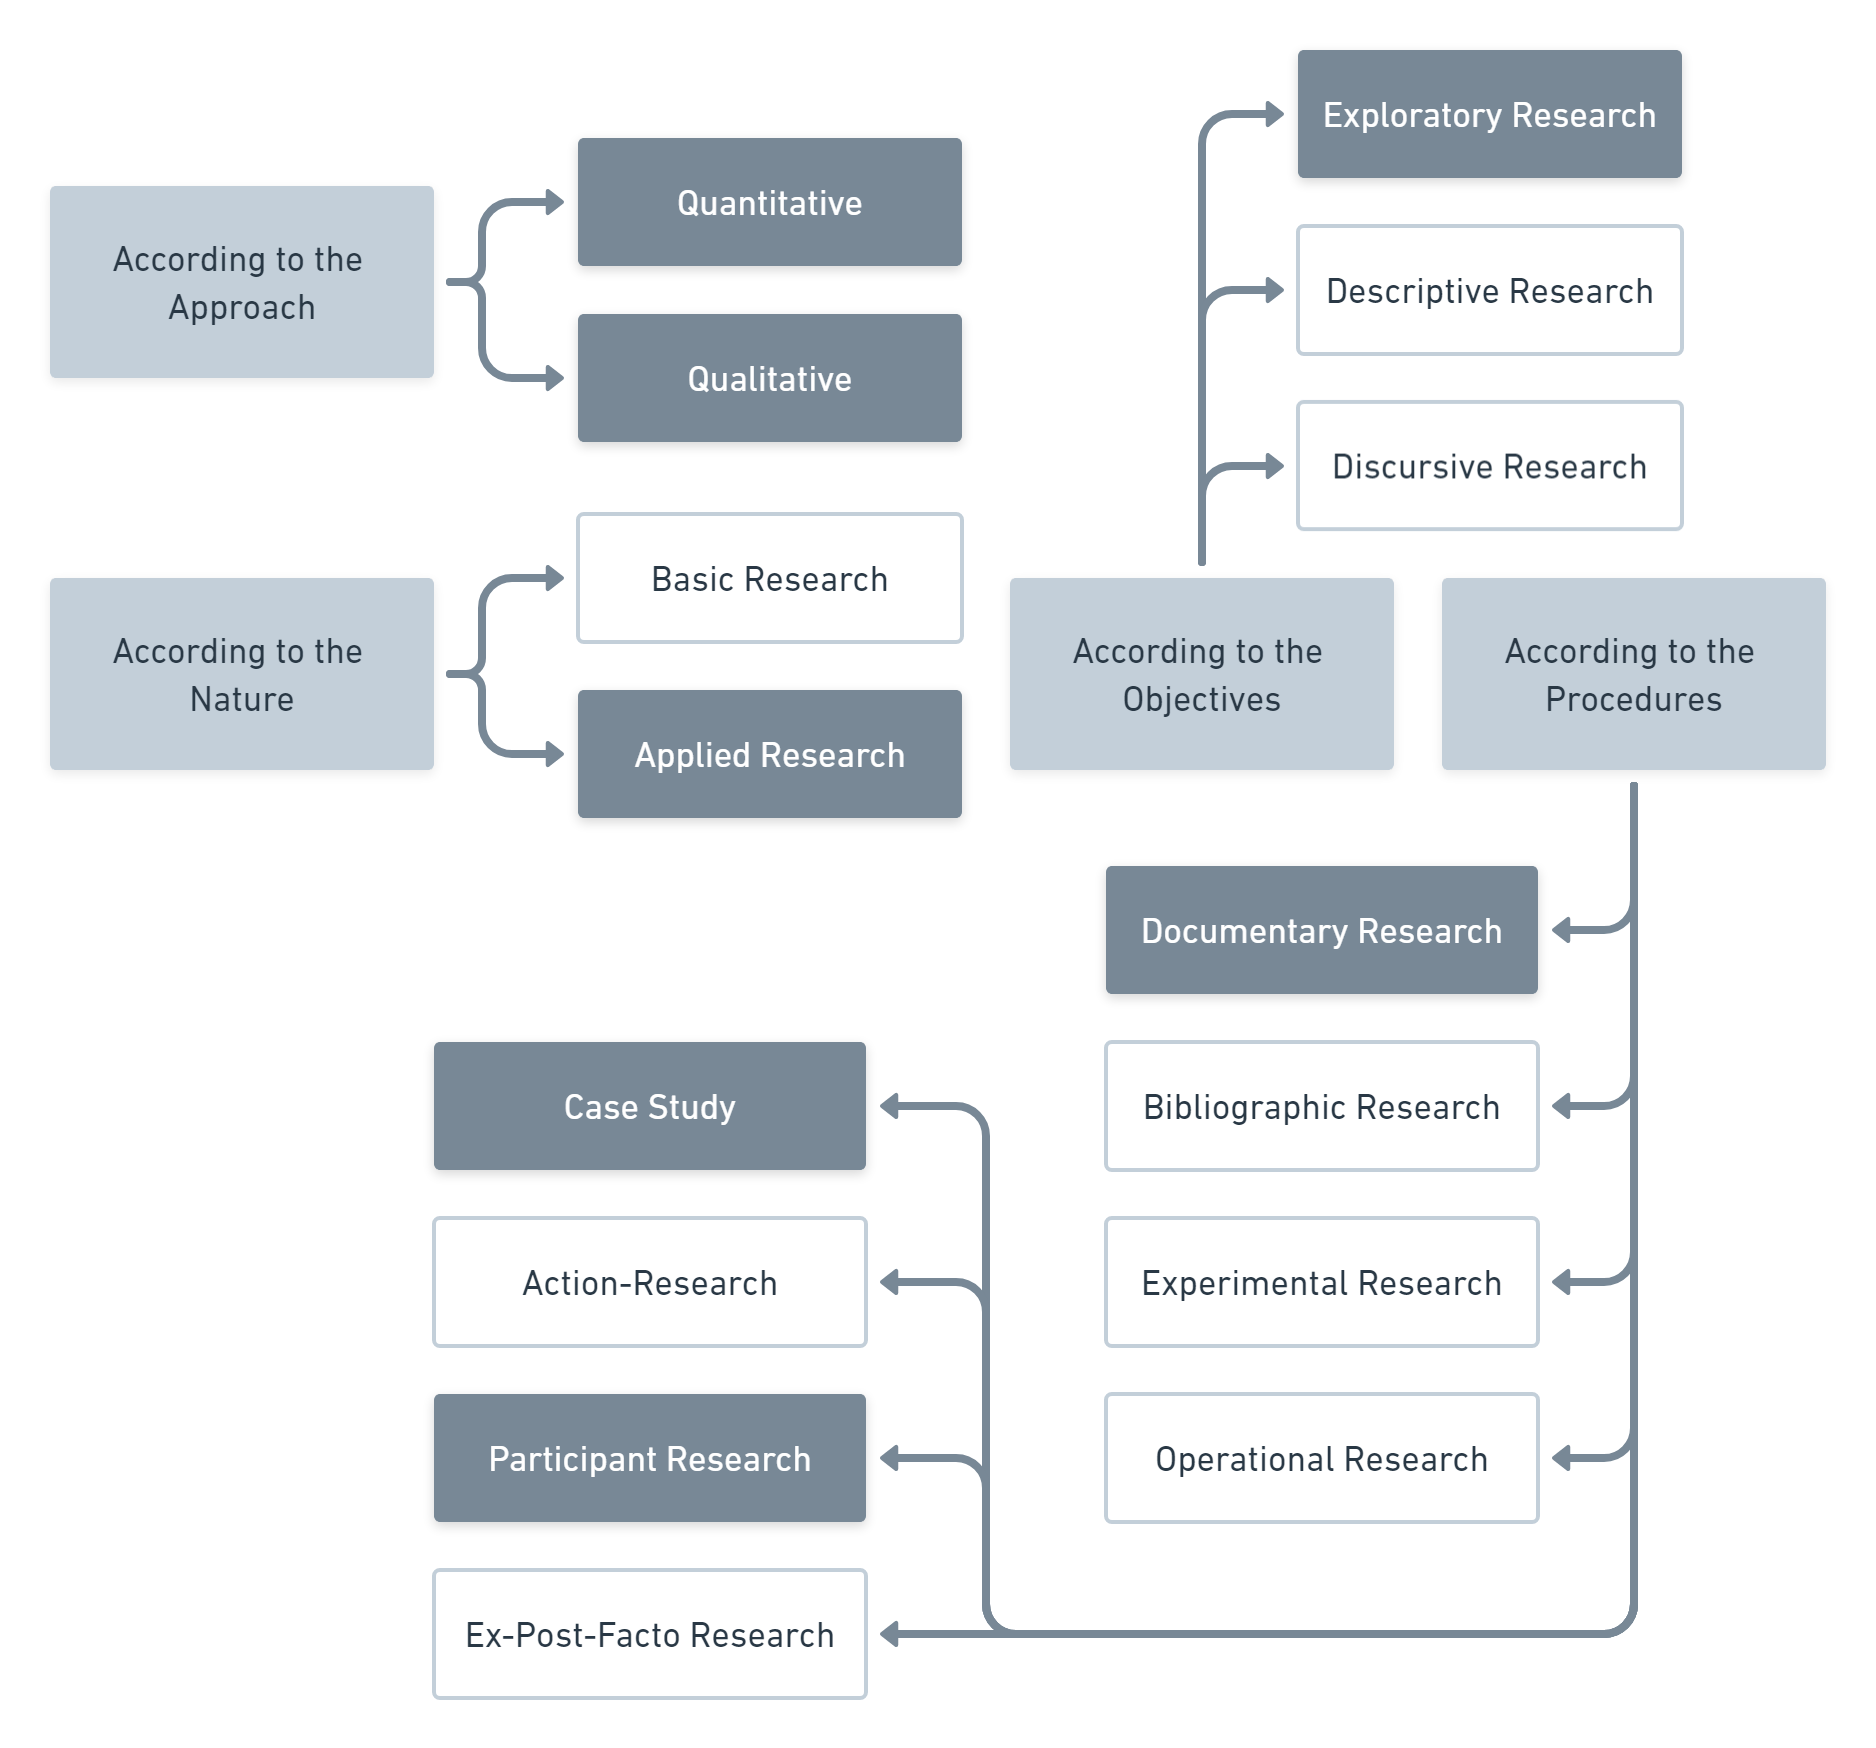
\includegraphics[width=16cm]{img/Research Classification@2x.png}
    \end{center}
    \fonte{Adapted from \cite{Prodanov:2013}.}
\end{figure}

Looking through the nature point of view, this is an \textbf{Applied Research}. It has the goal of generating knowledge to the solution of specific problems, through a practical application. It is related to local interests and often has a new process or product as a result.

From the objectives point of view, it is classified as an \textbf{Exploratory Research}, since one of its goals is to discover more information about what is being investigated, and maybe finding a new type of approach to the subject. This type of research generally takes the form of bibliographic research and \textbf{Case Studies}. The former doesn't apply to this study, though, because the final product won't be heavily inspired on white literature. Only the latter applies, because researches of this nature are more focused on the immediate application of knowledge in a circumstantial reality, emphasizing the development of theories.

However, the product will certainly be inspired by gray literature, meaning it fits as a \textbf{Documentary Research}. It is similar to bibliographic research, but the main difference between them is the nature of their sources. While bibliographic research makes fundamental use of contributions from various authors on a given subject, documentary research is based on materials that have not yet received an analytical treatment or that can be reworked according to the research objectives.

According to the technical procedures, this research fits in the \textbf{Participant Research}, because discovering the universe experienced by the population implies understanding, from an internal perspective, the point of view of individuals and groups about the situations they experience. Which will be achieved through a survey, described in more detail in \autoref{survey}.

Through the approach point of view, the research is both \textbf{Quantitative}, meaning translating opinions and information into numbers to classify and analyze them. And also \textbf{Qualitative}, because some parts of the study can't be quantified, and must be understood subjectively. An example would be to receive written, detailed feedback from a target-user through the survey.

\section{Research Design}\label{sec:met-3}

In order to conduct the study correctly, a research design was created. The activities are grouped in five phases:
\begin{inparaenum}[(1)]
    \item gather information;
    \item begin development;
    \item write term paper;
    \item develop;
    \item evaluate.
\end{inparaenum}
They are all described in this section and can also be observed in \autoref{fig:research-design}.

\begin{figure}[htb]
    \caption{Research Design}\label{fig:research-design}
    \begin{center}
        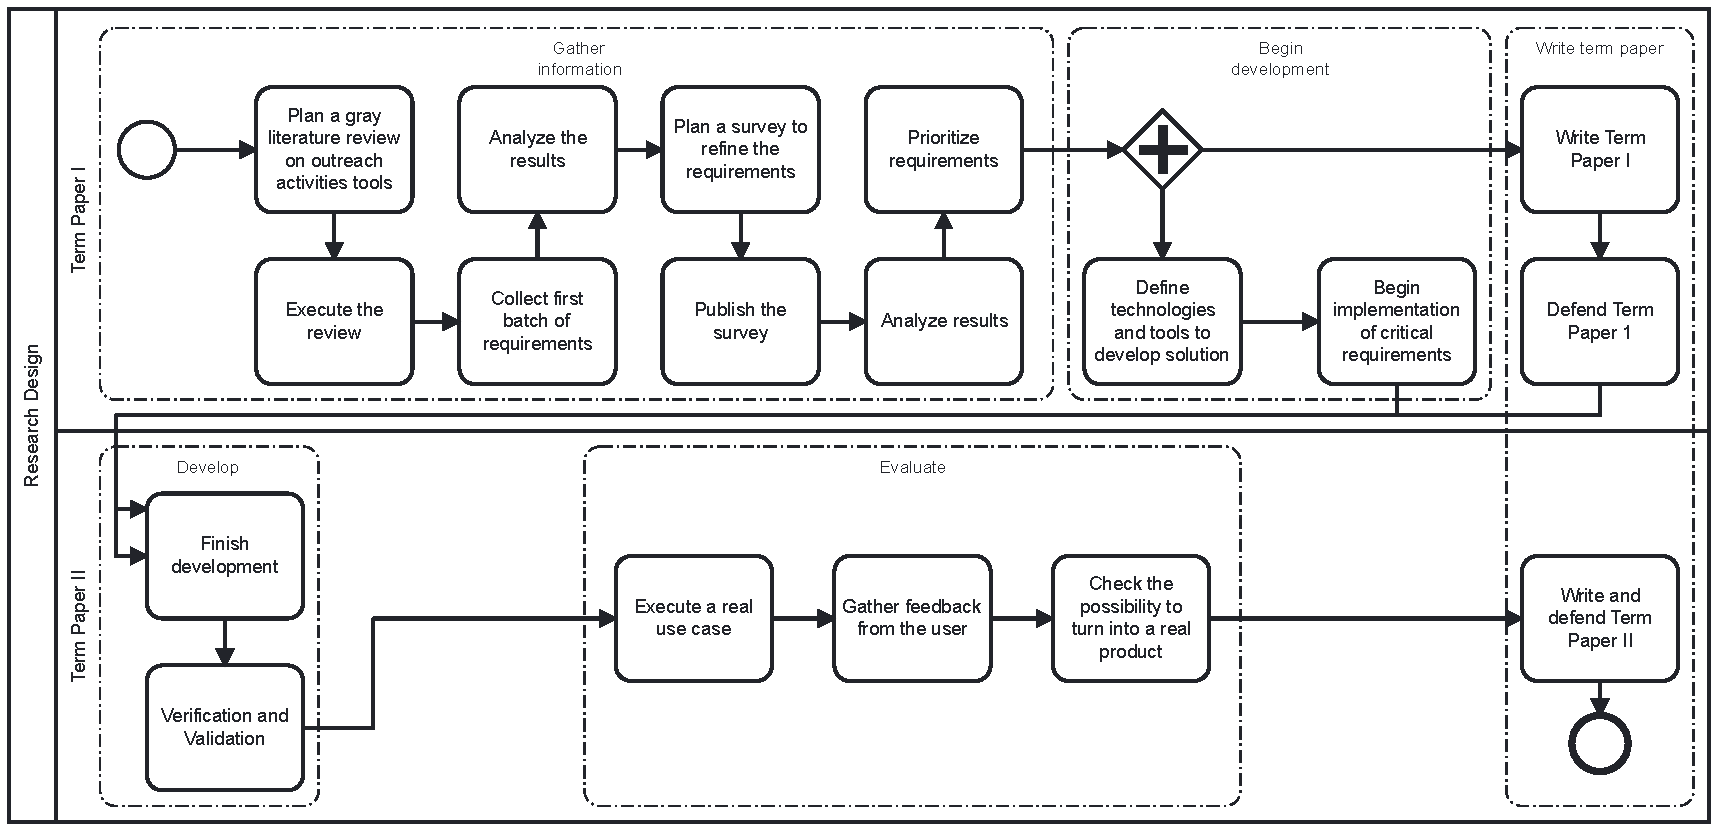
\includegraphics[width=16cm]{img/research design.pdf}
    \end{center}
    \fonte{Author.}
\end{figure}

The \textbf{gather information} group aims to create two tangible artifacts: the gray literature systematic review and the survey to better understand the scope of the goal product and most importantly collect a list of well defined requirements.

The \textbf{begin development} group is where the implementation and the term paper writing begins. This is where the technologies used throughout the development of the product are defined. The most important requirements should already be implemented as well.

Next, there is the \textbf{write term paper} group, in which both first and second term papers are going to be written and defended. It is important to notice that the first work will be written while the initial \ac{MVP} implementation is on going.

Continuing to the next milestone, is the \textbf{develop} group, where it is planned to finish the product development. After that, in the \textbf{evaluate} group, is where the real use case will be ran, and the feedback from it, analyzed. If all goes well, the product might turn into a real solution, adopted by the university to be used.

% Adicionar cronograma

\section{Chapter Summary}\label{sec:met-4}

This chapter provided an idea of how the methodology is defined for the study and how the research can be classified. In addition, the created research design was presented, showcasing the different planned processes for the future and those that have already been executed. The \autoref{background} describes all the information and background necessary for the success of this work, while also assisting the reader in better understanding the research methodology previously described.

% %------------------------------------------------------------------------------
% \section{Citações}
% %------------------------------------------------------------------------------

% \index{citações!diretas}Utilize o ambiente \texttt{citacao} para incluir citações diretas com mais de três linhas:

% \begin{citacao}
% As citações diretas, no texto, com mais de três linhas, devem ser destacadas com recuo de 4 cm da margem esquerda, com letra menor que a do texto utilizado e sem as aspas.
%   No caso de documentos datilografados, deve-se observar apenas o recuo \cite[5.3]{NBR10520:2002}
% \end{citacao}

% \index{citações!simples}Citações simples, com até três linhas, devem ser incluídas com aspas.
%   Observe que em \LaTeX~as aspas iniciais são diferentes das finais: ``Amor é fogo que arde sem se ver''.

% Para as citações indiretas, o comando padrão, \verb|\cite|, realiza a forma mais comum de citação \cite{SisbiUnipampa2011}.
%   A outra das formas mais usadas, para citar em texto corrido, é conseguida com o comando \verb|\citeonline|: segundo \citeonline{SisbiUnipampa2011}, na citação indireta, o número da página é opcional.


% %------------------------------------------------------------------------------
% \subsection{Referências internas}\label{sec:referencias_internas}
% %------------------------------------------------------------------------------

% Usa-se o comando \verb|\ref{}| para referenciar uma Tabela ou Figura.
%   Por exemplo, esta é uma referência para a Tabela~\ref{tab:nivinv}.
%   Mas também pode-se usar o comando \verb|\autoref{}|, que insere o tipo também.
%   Por exemplo, esta é outra referência para a \autoref{tab:nivinv}.

% Há vários outros comandos interessantes.
%   Eles estão no fonte do \autoref{introducao}, na \autoref{sec:referencias_internas}
%   \footnote{O número do capítulo indicado é \ref{introducao}, que se inicia à página \pageref{introducao}.}
%   (\nameref{introducao}, \autopageref{introducao}).


% %------------------------------------------------------------------------------
% \section{Tabelas}
% %------------------------------------------------------------------------------

% \index{tabelas}A \autoref{tab:nivinv} é um exemplo de tabela construída em \LaTeX.
%   Como sugestão de formatação, evite ao máximo o uso de linhas verticais.
%   As colunas de uma tabela devem ser separadas visivelmente.
%   O contrário indica que a tabela está mal formatada ou que certas informações não deveriam estar nela.

% Da mesma forma, evite o uso de linhas horizontais para separar linhas da tabela.
%   Use-as apenas para separar o cabeçalho e eventuais partes importantes.
%   Para obter um resultado ainda mais elegante, use os comandos do pacote \texttt{booktabs}.

% Veja essas sugestões aplicas na \autoref{tab:nivinv}.

% \begin{table}[!htb]
%   \footnotesize
%   \caption[Níveis de investigação]{Níveis de investigação.}
%   \label{tab:nivinv}
%   \begin{tabular}{m{2.6cm}m{6.0cm}m{2.25cm}m{3.40cm}}
%     \toprule
%     \textbf{Nível de Investigação} & \textbf{Insumos}                                                   & \textbf{Sistemas de Investigação} & \textbf{Produtos}    \\
%     \midrule
%     Meta-nível                     & Filosofia\index{filosofia} da Ciência                              & Epistemologia                     & Paradigma            \\
%     Nível do objeto                & Paradigmas do metanível e evidências do nível inferior             & Ciência                           & Teorias e modelos    \\
%     Nível inferior                 & Modelos e métodos do nível do objeto e problemas do nível inferior & Prática                           & Solução de problemas \\
%     \bottomrule
%   \end{tabular}
%   \fonte{\citeonline{van86}}
% \end{table}


% Uma opção avançada para a criação de tabelas é usar o pacote \texttt{pgfplotstable}.
%   Ele permite que os dados de um arquivo sejam lidos e colocados em uma tabela, formatando-os da maneira que se quiser.
%   A \autoref{tab:dados} é um exemplo.
%   Veja o arquivo \texttt{desenvolvimento.tex} para os comandos necessários.

% % Necessário o pacote filecontents
% % Especifica o conteúdo que será gravado no dado arquivo (nesse caso, resultados.txt)
% \begin{filecontents*}{resultados.txt}
% tamanho metodo1 metodo2 metodo3
% 10  30    36.2  28.3
% 20  54.8  52.5  56.8
% 30  65    59.6  74.1
% 40  64.5  59.6  76.7
% 50  64.6  59.6  76.5
% \end{filecontents*}

% % Para definir os estilos das colunas e da tabela
% \pgfplotstableset{
%      %columns={tamanho,metodo1,{grad(log(metodo2),log(metodo3))}},
%      columns/metodo1/.style={
%          column name=\textsc{Método 1 (\%)},
%          column type=c,
%          %dec sep align={c},
%          %sci,sci zerofill,sci subscript,
%          fixed,fixed zerofill,
%          precision=1},
%      columns/metodo2/.style={
%          column name=\textsc{Método 2 (\%)},
%          column type=c,
%          fixed,fixed zerofill,precision=1},
%      columns/metodo3/.style={
%          column name=\textsc{Método 3 (\%)},
%          fixed,fixed zerofill,precision=1},
%      columns/media/.style={
%          column name=\textsc{Média (\%)},
%          fixed,fixed zerofill,precision=1},
%      create on use/media/.style={
%          create col/expr={(\thisrow{metodo1}+\thisrow{metodo2}+\thisrow{metodo3})/3}},
%      every head row/.style={
%          before row=\toprule,after row=\midrule},
%      every last row/.style={
%          after row=\bottomrule}}

% \begin{table}[!phtb]
%   \caption{Exemplo de tabela com dados de arquivo.}
%   \label{tab:dados}
%   \begin{center}
%     % Lê do arquivo resultados.txt as colunas especificadas e as formata de acordo com
%     % os estilos acima ou com os estilos especificados aqui (nesse caso, para a coluna tamanho).
%     \pgfplotstabletypesetfile[
%       columns={tamanho,metodo1,metodo2,metodo3,media},
%       columns/tamanho/.style={column name=\textsc{Tamanho}}
%     ]{resultados.txt}
%   \end{center}
% \end{table}


% %------------------------------------------------------------------------------
% \section{Figuras}
% %------------------------------------------------------------------------------

% \index{figuras}Figuras podem ser criadas diretamente em \LaTeX.
%   Uma das melhores formas, por ser relativamente simples, bem documentada e gerar ótimos resultados, é com o uso do pacote tikz\footnote{Há vários exemplos em \url{http://www.texample.net/}.}.
%   Ele permite gerar diagramas, árvores, fluxogramas etc.
%   A \autoref{fig:fib} mostra um exemplo simples de árvore.

% \begin{figure}[!htb]
%   \caption{Árvore de recursão de Fibonacci.}\label{fig:fib}
%   \begin{center}
%   \begin{tikzpicture}[level/.style={sibling distance=160mm/(2^#1)},
%                       level 4/.style={sibling distance=18mm},
%                       every node/.style={minimum width=5mm}]
%     \node [circle,draw] (z) {$fib(5)$}
%       child {node [circle,draw] (a) {$fib(4)$}
%         child {node [circle,draw] (b) {$fib(3)$}
%           child {node [circle,draw=red] (c) {$fib(2)$}
%             child {node [circle,draw] (d) {$fib(1)$}}
%             child {node [circle,draw] (e) {$fib(0)$}}
%           }
%           child {node [circle,draw] (f) {$fib(1)$}}
%         }
%         child {node [circle,draw=red] (g) {$fib(2)$}
%           child {node [circle,draw] (h) {$fib(1)$}}
%           child {node [circle,draw] (i) {$fib(0)$}}
%         }
%       }
%       child {node [circle,draw] (j) {$fib(3)$}
%         child {node [circle,draw=red] (k) {$fib(2)$}
%           child {node [circle,draw] (l) {$fib(1)$}}
%           child {node [circle,draw] (m) {$fib(0)$}}
%         }
%         child {node [circle,draw] (n) {$fib(1)$}}
%       };
%   \end{tikzpicture}
%   \end{center}
% \end{figure}

% Junto com o pacote pgfplots também é possível gerar gráficos de funções ou a partir de dados em um arquivo (como no caso da \autoref{tab:dados}).
%   As Figuras \ref{fig:grafico1} e \ref{fig:grafico2} mostram exemplos de gráficos de função, e a \autoref{fig:grafico_dados} um exemplo de gráfico a partir dos mesmos dados que os da \autoref{tab:dados}.

% \begin{figure}[!htb]
%   \caption{Gráfico produzido diretamente no arquivo fonte.}\label{fig:grafico1}
%   \begin{center}
%   \begin{tikzpicture}[scale=1]
%   \begin{axis}[
%       width=.65\textwidth,
%       ymin=0,xmin=0,xmax=1000,
%       xlabel=$n$,ylabel=$T(n)$,
%       ylabel near ticks,
%       scaled ticks=false, % Evita o uso de notação exponencial 10^2
%       ticklabel style={/pgf/number format/.cd,fixed,use comma,1000 sep={}}, % Para vírgula como separador decimal
%       legend pos=outer north east,
%       legend style={draw=none},
%     ]
%     \addplot[blue,thick,domain=1:1000] {1 * x * ln(x) / ln(2)} node[near end,above] {$g(n)$};
%     \addplot[green,thick,domain=1:1000] {12 * x * ln(x) / ln(2)} node[near end,above left] (g) {$12g(n)$};
%     \addplot[orange,thick,domain=1:1000] {5 * x * ln(x) / ln(2) + 21000} node[near end,above] {$f(n)$};
%     \addplot+[red,very thick,dashed,mark=o,const plot,samples at=354] {12 * x * ln(x) / ln(2)};
%     \addplot[red,thick,dashed,const plot] coordinates {(354,0) (354,35970)};
%     %\addlegendentry{$g(n)$}; %{$n \lg(n)$}
%     %\addlegendentry{$12g(n)$}; %{$12n \lg(n)$}
%     %\addlegendentry{$f(n)$};
%     \draw[black!70,very thin,solid,text=black] (axis cs:354,35970) -- (axis cs:250,50000) node[above] {$n_0\approx 354$};
%     \draw[black!70,very thin,solid,text=black] (g.west) -> (axis cs:400,90000) node[below] {$c=12$};
%   \end{axis}
%   \end{tikzpicture}
%   \end{center}
% \end{figure}

% \begin{figure}[!htb]
%   \caption{Outro gráfico feito em \LaTeX.}
%   \label{fig:grafico2}
%   \begin{center}
%   \begin{tikzpicture}
%   \begin{axis}[
%       width=.8\textwidth,
%       ymin=0,xmin=0,xmax=150,
%       xlabel=$n$,ylabel=$T(n)$,
%       ylabel near ticks,
%       scaled ticks=false, % Evita o uso de notação exponencial 10^2
%       yticklabel style={/pgf/number format/.cd,fixed,use comma,1000 sep={}}, % Para vírgula como separador decimal
%       legend pos=north west,
%       legend style={draw=none},
%     ]
%     \addplot[blue,mark=*,thick,domain=1:150] {6 * x * ln(x) / ln(2) + 6 * x};
%     \addplot[orange,mark=square,thick,domain=1:150] {1 / 2 * x^2};
%     \addlegendentry{$6n \lg(n) + 6n$}
%     \addlegendentry{$\frac{1}{2}n^2$}
%   \end{axis}
%   \end{tikzpicture}
%   \end{center}
% \end{figure}


% \begin{figure}[!htb]
%   \caption{Variação dos resultados utilizando seleção por Janela Deslizante.}
%   \label{fig:grafico_dados}
%   \begin{center}
%   \begin{tikzpicture}[scale=1]
%     \begin{axis}[
%       width=0.9\textwidth,%height=0.6\textwidth,
%       xmode=normal,ymode=normal,
%       ymin=20,
%       xtick=data,%ticks=both,
%       xlabel=Tamanho,
%       ylabel=Acerto (\%),
%       legend pos=south east,
%       %legend style={draw=none},
%     ]
%     \addplot+[thick] table [x=tamanho,y=metodo1,header=true] {resultados.txt};
%     \addlegendentry{Método 1}
%     \addplot+[thick,mark=square] table [x=tamanho,y=metodo2,header=true] {resultados.txt};
%     \addlegendentry{Método 2}
%     \addplot+[thick,mark=triangle] table [x=tamanho,y=metodo3,header=true] {resultados.txt};
%     \addlegendentry{Método 3}
%   \end{axis}
%   \end{tikzpicture}
% \end{center}
% \end{figure}


% Figuras também podem ser incorporadas de arquivos externos, como é o caso da \autoref{fig:grafico_excel}.
%   Se a figura que ser incluída se tratar de um diagrama, um gráfico ou uma ilustração que você mesmo produza, priorize o uso de imagens vetoriais no formato PDF.
%   Com isso, o tamanho do arquivo final do trabalho será menor, e as imagens terão uma apresentação melhor, principalmente quando impressas, uma vez que imagens vetorias são perfeitamente escaláveis para qualquer dimensão.
%   Nesse caso, se for utilizar o Microsoft Excel para produzir gráficos, ou o Microsoft Word para produzir ilustrações, exporte-os como PDF e os incorpore ao documento conforme o exemplo abaixo.
%   No entanto, para manter a coerência no uso de software livre (já que você está usando \LaTeX e \abnTeX), teste a ferramenta \textsf{InkScape}\index{InkScape}\footnote{\url{http://inkscape.org/}}.
%   Ela é uma excelente opção de código-livre para produzir ilustrações vetoriais, similar ao CorelDraw\index{CorelDraw} ou ao Adobe Illustrator\index{Adobe Illustrator}.

% De todo modo, caso não seja possível utilizar arquivos de imagens como PDF, utilize qualquer outro formato, como PNG, JPEG, etc.
%   Nesse caso, você pode tentar aprimorar as imagens incorporadas com o software livre \textsf{Gimp}\index{Gimp}\footnote{\url{http://www.gimp.org/}}.
%   Ele é uma alternativa livre ao Adobe Photoshop\index{Adobe Photoshop}.

% \begin{figure}[htb]
%   \caption{Gráfico produzido em Excel e salvo como PDF.}\label{fig:grafico_excel}
%   \begin{center}
%       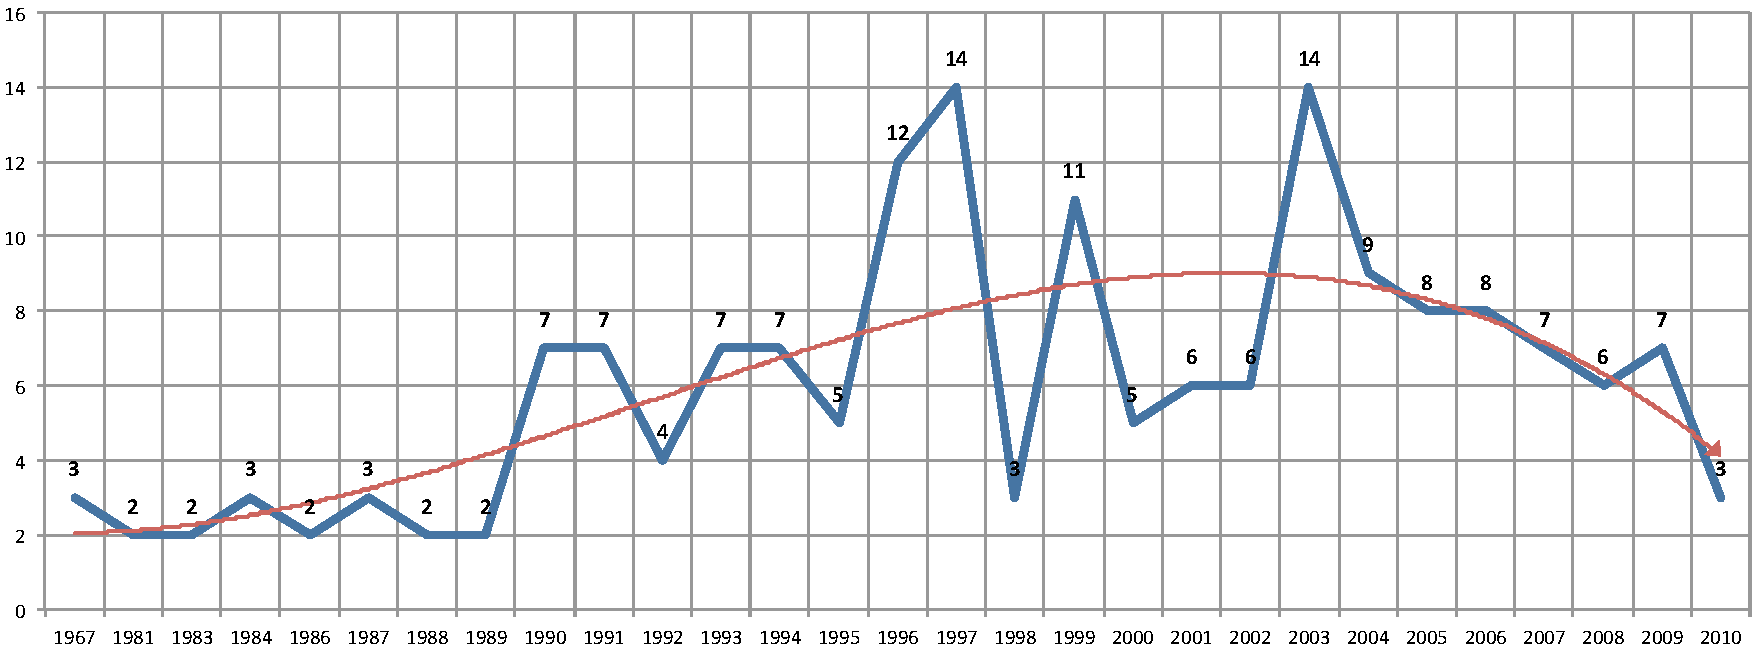
\includegraphics[scale=0.5]{img/abntex2-modelo-img-grafico}
%   \end{center}
%   \fonte{\citeonline[p. 24]{araujo2012}}
% \end{figure}


% A \autoref{fig:exemplo} na página \pageref{fig:exemplo} contém duas subfiguras, \autoref{subfig:exemplo:arquivo} e \subcaptionref{subfig:exemplo:tikz}.
%   A \autoref{subfig:exemplo:arquivo} foi inserida de um arquivo externo, enquanto a \autoref{subfig:exemplo:tikz} foi escrita dentro do próprio código \TeX.
%   A \autoref{fig:exemplo2} contém o mesmo exemplo, mas usando comandos diferentes para inserir as Subfiguras \ref{subfig:exemplo2:arquivo} e \subcaptionref{subfig:exemplo2:tikz}.

% \begin{figure}[!htb]
%   \centering
%   \caption{Exemplo de subfiguras.}\label{fig:exemplo}
%   \subbottom[Uma figura de um arquivo.]{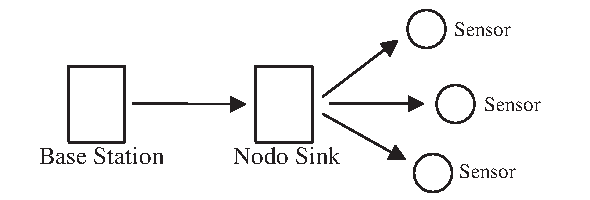
\includegraphics[scale=1]{img/exemplo}\label{subfig:exemplo:arquivo}}\fonte{\citeonline{Moro2012}}
%   \qquad
%   \subbottom[Uma figura em puro código TikZ.]{%
%     \begin{tikzpicture}
%       [tipo1/.style={rectangle,draw,minimum height=13mm,minimum width=9mm},
%       tipo2/.style={circle,draw,minimum height=6mm,minimum width=6mm,
%                      prefix after command={\pgfextra{\tikzset{every label/.style={font=\footnotesize}}}}},
%       tiposeta/.style={->,shorten >=6pt,shorten <=6pt,>=triangle 60,thick}]
%       \node [tipo1] (base) [label=below:Base Station] {};
%       \node [tipo1] (sink) [right=22mm of base,label=below:Nodo Sink] {};
%       \node [tipo2] (sensor1) [above right=4mm and 17mm of sink,label=right:Sensor] {};
%       \node [tipo2] (sensor2) [right=22mm of sink,label=right:Sensor] {};
%       \node [tipo2] (sensor3) [below right=4mm and 17mm of sink,label=right:Sensor] {};
%       \draw [tiposeta] (base.east) -- (sink.west);
%       \draw [tiposeta] (sink.east) -- (sensor1.south west);
%       \draw [tiposeta] (sink.east) -- (sensor2.west);
%       \draw [tiposeta] (sink.east) -- (sensor3.north west);
%     \end{tikzpicture}
%     \label{subfig:exemplo:tikz}%
%   }
%   \legend{Alterado: de \citeonline{Moro2012}}%
% \end{figure}

% Na \autoref{fig:exemplo}, as legendas (que indicam a fonte) para cada subfigura só funcionaram porque as figuras ficaram uma embaixo da outra.
%   Se elas estivessem lado a lado, a inserção do comando \verb|\legend| em cada uma faria com que elas ficassem organizadas na vertical.
%   Uma legenda geral funcionaria, entretanto.

% Na \autoref{fig:exemplo2}, tanto legendas para subfiguras quanto uma legenda geral funcionam.

% \begin{figure}[!htb]
%   \centering
%   \caption{Mesmo exemplo de subfiguras, agora em escala.}\label{fig:exemplo2}
%   \begin{minipage}{0.48\textwidth}
%     \centering
%     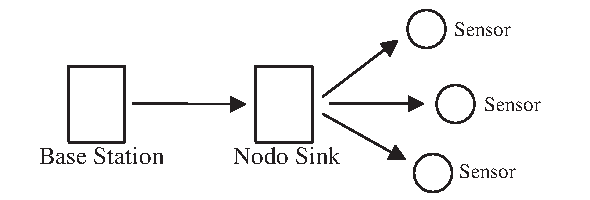
\includegraphics[scale=.5]{img/exemplo}
%     \subcaption{Uma figura de um arquivo.\label{subfig:exemplo2:arquivo}}
%     \fonte{\citeonline{Moro2012}}%
%   \end{minipage}
%   %\quad
%   \begin{minipage}{0.48\textwidth}
%     \centering
%     \resizebox{0.6\textwidth}{!}{%
%       \begin{tikzpicture}[%
%          tipo1/.style={rectangle,draw,minimum height=13mm,minimum width=9mm},
%          tipo2/.style={circle,draw,minimum height=6mm,minimum width=6mm,
%                       prefix after command={\pgfextra{\tikzset{every label/.style={font=\footnotesize}}}}},
%          tiposeta/.style={->,shorten >=6pt,shorten <=6pt,>=triangle 60,thick}]
%         \node [tipo1] (base) [label=below:Base Station] {};
%         \node [tipo1] (sink) [right=22mm of base,label=below:Nodo Sink] {};
%         \node [tipo2] (sensor1) [above right=4mm and 17mm of sink,label=right:Sensor] {};
%         \node [tipo2] (sensor2) [right=22mm of sink,label=right:Sensor] {};
%         \node [tipo2] (sensor3) [below right=4mm and 17mm of sink,label=right:Sensor] {};
%         \draw [tiposeta] (base.east) -- (sink.west);
%         \draw [tiposeta] (sink.east) -- (sensor1.south west);
%         \draw [tiposeta] (sink.east) -- (sensor2.west);
%         \draw [tiposeta] (sink.east) -- (sensor3.north west);
%       \end{tikzpicture}
%     }
%     \subcaption{\label{subfig:exemplo2:tikz}Uma figura em puro código TikZ.}
%     \fonte{Alterado de \citeonline{Moro2012}}%
%   \end{minipage}
%   \fonte{Fonte geral}%
% \end{figure}


% %------------------------------------------------------------------------------
% \subsection{Sobre a indicação da fonte de uma tabela ou figura}
% %------------------------------------------------------------------------------

% As normas \citeonline[5.8]{NBR14724:2011} e o Manual de Normatização da UNIPAMPA \cite{SisbiUnipampa2011} dizem para, ``Após a ilustração, na parte inferior, indicar a fonte consultada (elemento obrigatório, mesmo que seja produção do próprio autor), legenda, notas e outras informações necessárias à sua compreensão (se houver).''
%   A primeira interpretação é a de que, mesmo que o autor tenha criado a figura, a fonte deverá ser indicada.
%   Com efeito, várias outras normas, manuais e inclusive o exemplo do pacote \abnTeX2 usam ``Fonte: os autores'' em alguns lugares.

% Entretanto, isso não está correto.
%   Veja o trecho em destaque: ``Após a ilustração, na parte inferior, indicar a fonte \textbf{consultada} (elemento obrigatório, mesmo que seja produção do próprio autor) (...).''
%   A interpretação correta é a de que, caso a ilustração tenha sido \textbf{extraída} de um documento, a fonte deve ser indicada, ainda que esse documento pertença ao próprio autor.
%   A sentença original das normas deveria ter sido melhor escrita para evitar a interpretação incorreta.

% Assim, não indique a fonte se a figura ou tabela for original, ou seja, foi criada para o trabalho.
%   Caso contrário, indique a fonte.
%   Mas cuidado: caso a figura ou tabela tenha sido adaptada de outra já publicada, então é obrigatório indicar ``adaptado de'' ou ``acrescida de'' seguido da referência da fonte de onde ela foi extraída.


% %------------------------------------------------------------------------------
% \section{Expressões matemáticas}
% %------------------------------------------------------------------------------

% \index{expressões matemáticas}Use o ambiente \texttt{equation} para escrever expressões matemáticas numeradas:

% \begin{equation}
%   \forall x \in X, \quad \exists \: y \leq \epsilon
% \end{equation}

% Escreva expressões matemáticas entre \$ e \$, como em $\lim_{x \to \infty} \exp(-x) = 0$, para que fiquem na mesma linha.

% Também é possível usar colchetes para indicar o início de uma expressão matemática que não é numerada.

% \[
% \left|\sum_{i=1}^n a_ib_i\right|
% \le
% \left(\sum_{i=1}^n a_i^2\right)^{1/2}
% \left(\sum_{i=1}^n b_i^2\right)^{1/2}
% \]

% Consulte mais informações sobre expressões matemáticas em \url{http://code.google.com/p/abntex2/w/edit/Referencias}.


% %------------------------------------------------------------------------------
% \section{Enumerações: alíneas e subalíneas}
% %------------------------------------------------------------------------------

% \index{alíneas}\index{subalíneas}\index{incisos}Quando for necessário enumerar os diversos assuntos de uma seção que não possua título, esta deve ser subdividida em alíneas \cite[4.2]{NBR6024:2012}:

% \begin{alineas}

%   \item os diversos assuntos que não possuam título próprio, dentro de uma mesma
%   seção, devem ser subdivididos em alíneas\footnote{As notas devem ser digitadas ou datilografadas
%   dentro das margens, ficando separadas do texto por um espaço simples de entre as
%   linhas e por filete de 5 cm, a partir da margem esquerda. Devem ser
%   alinhadas, a partir da segunda linha da mesma nota, abaixo da primeira letra
%   da primeira palavra, de forma a destacar o expoente, sem espaço entre elas e
%   com fonte menor. \citeonline[5.2.1]{NBR14724:2011}};

%   \item o texto que antecede as alíneas termina em dois pontos;
%   \item as alíneas devem ser indicadas alfabeticamente, em letra minúscula, seguida de parêntese. Utilizam-se letras dobradas, quando esgotadas as letras do alfabeto;

%   \item as letras indicativas das alíneas devem apresentar recuo em relação à
%   margem esquerda;

%   \item o texto da alínea deve começar por letra minúscula e terminar em
%   ponto-e-vírgula, exceto a última alínea que termina em ponto final;

%   \item o texto da alínea deve terminar em dois pontos, se houver subalínea;

%   \item a segunda e as seguintes linhas do texto da alínea começa sob a
%   primeira letra do texto da própria alínea;

%   \item subalíneas \cite[4.3]{NBR6024:2012} devem ser conforme as alíneas a
%   seguir:

%   \begin{alineas}
%      \item as subalíneas devem começar por travessão seguido de espaço;

%      \item as subalíneas devem apresentar recuo em relação à alínea;

%      \item o texto da subalínea deve começar por letra minúscula e terminar em
%      ponto-e-vírgula. A última subalínea deve terminar em ponto final, se não
%      houver alínea subsequente;

%      \item a segunda e as seguintes linhas do texto da subalínea começam sob a
%      primeira letra do texto da própria subalínea.
%   \end{alineas}

%   \item no \abnTeX\ estão disponíveis os ambientes \texttt{incisos} e \texttt{subalineas}, que em suma são o mesmo que se criar outro nível de \texttt{alineas}, como nos exemplos à seguir:

%   \begin{incisos}
%     \item \textit{Um novo inciso em itálico};
%   \end{incisos}

%   \item Alínea em \textbf{negrito}:

%   \begin{subalineas}
%     \item \textit{Uma subalínea em itálico};
%     \item \underline{\textit{Uma subalínea em itálico e sublinhado}};
%   \end{subalineas}

%   \item Última alínea com \emph{ênfase}.

% \end{alineas}


% %------------------------------------------------------------------------------
% \section{Espaçamento entre parágrafos e linhas}
% %------------------------------------------------------------------------------

% \index{espaçamento!dos parágrafos}O tamanho do parágrafo, espaço entre a margem e o início da frase do parágrafo, é definido por:

% \begin{verbatim}
%   \setlength{\parindent}{1.3cm}
% \end{verbatim}

% \index{espaçamento!do primeiro parágrafo}Por padrão, não há espaçamento no primeiro parágrafo de cada início de divisão do documento (\autoref{sec:divisoes}).
%   Porém, você pode definir que o primeiro parágrafo também seja indentado, como é o caso deste documento.
%   Para isso, apenas inclua o pacote \textsf{indentfirst} no preâmbulo do documento:
% \begin{verbatim}
%   \usepackage{indentfirst}      % Indenta o primeiro parágrafo de cada seção.
% \end{verbatim}

% \index{espaçamento!entre os parágrafos}O espaçamento entre um parágrafo e outro pode ser controlado por meio do comando:
% \begin{verbatim}
%   \setlength{\parskip}{0.2cm}  % tente também \onelineskip
% \end{verbatim}

% \index{espaçamento!entre as linhas}O controle do espaçamento entre linhas é definido por:
% \begin{verbatim}
%   \OnehalfSpacing       % espaçamento um e meio (padrão);
%   \DoubleSpacing        % espaçamento duplo
%   \SingleSpacing        % espaçamento simples
% \end{verbatim}

% Para isso, também estão disponíveis os ambientes:
% \begin{verbatim}
%   \begin{SingleSpace} ...\end{SingleSpace}
%   \begin{Spacing}{hfactori} ... \end{Spacing}
%   \begin{OnehalfSpace} ... \end{OnehalfSpace}
%   \begin{OnehalfSpace*} ... \end{OnehalfSpace*}
%   \begin{DoubleSpace} ... \end{DoubleSpace}
%   \begin{DoubleSpace*} ... \end{DoubleSpace*}
% \end{verbatim}

% Para mais informações, consulte \citeonline[p. 47-52 e 135]{memoir}.


% %------------------------------------------------------------------------------
% \section{Inclução de outros arquivos}\label{sec:include}
% %------------------------------------------------------------------------------

% É uma boa prática dividir o seu documento em diversos arquivos, e não apenas escrever tudo em um único.
%   Esse recurso foi utilizado neste documento.
%   Para incluir diferentes arquivos em um arquivo principal, de modo que cada arquivo incluído fique em uma página diferente, utilize o comando:
% \begin{verbatim}
%   \include{documento-a-ser-incluido}      % sem a extensão .tex
% \end{verbatim}

% Para incluir documentos sem quebra de páginas, utilize:
% \begin{verbatim}
%   \input{documento-a-ser-incluido}      % sem a extensão .tex
% \end{verbatim}


% %------------------------------------------------------------------------------
% \section{Compilar o documento \LaTeX}
% %------------------------------------------------------------------------------

% Geralmente os editores \LaTeX, como o TeXlipse\footnote{\url{http://texlipse.sourceforge.net/}}, o Texmaker\footnote{\url{http://www.xm1math.net/texmaker/}}, entre outros, compilam os documentos automaticamente, de modo que você não precisa se preocupar com isso.

% No entanto, você pode compilar os documentos \LaTeX usando os seguintes comandos, que devem ser digitados no \emph{Prompt de Comandos} do Windows ou no \emph{Terminal} do Mac ou do Linux:
% \begin{verbatim}
%   pdflatex ARQUIVO_PRINCIPAL.tex
%   bibtex ARQUIVO_PRINCIPAL.aux
%   makeindex ARQUIVO_PRINCIPAL.idx
%   makeindex ARQUIVO_PRINCIPAL.nlo -s nomencl.ist -o ARQUIVO_PRINCIPAL.nls
%   pdflatex ARQUIVO_PRINCIPAL.tex
%   pdflatex ARQUIVO_PRINCIPAL.tex
% \end{verbatim}
 % [OBRIGATORIO]
% Background - extensão universitária no Brasil, curricularização da extensão, soluções/ferramentas de apoio à extensão, leis federais, resoluções unipampa, implantação da extensão, tipos de extensão, perfis de pessoas envolvidas na extensão, programas e projetos de extensão na unipampa
% Unipampa Cidadã
%==============================================================================
\chapter{Background}\label{background}
%==============================================================================

In this chapter, information that complement the objective of the study are discussed, helping to understand the policies and resolutions involved. In \autoref{sec:bac-1} the national outreach activity policy will be presented, which is valid for all universities in Brazil. It applies for each \ac{OA} regarding its relation to the academic and external community. Soon after in \autoref{sec:bac-2-0} and \autoref{sec:bac-2} the vision of how both the \ac{ICES} as a whole and \acl{UNIPAMPA}, respectively, adapted to receive these new rules is described. Afterwards, in \autoref{sec:bac-3} the differences between outreach programs and projects will be presented, followed by a more detailed explanation about the ``\ac{UNIPAMPA} Cidadã'' project in \autoref{sec:bac-4}. The \autoref{sec:bac-5} showcases current available tools and solutions in the market which are related to the study goal product. The \autoref{sec:bac-6} reveals some tools related to the subject of the work, their commonalities and a high-level description. Finally in \autoref{sec:bac-7} a general summary of the chapter is presented.

\section{Outreach activities in Brazil}\label{sec:bac-1}

It is clear that participating in outreach activities has many benefits for the students who decide to take part in it \cite{sellou2011many}. Besides promoting individual growth, the activities can also serve as a bridge connecting students and professors even more. In order to preserve them and encourage younger students to participate in them, the \acl{FORPROEX} (\ac{FORPROEX}), updated the old version of the National Outreach Policy document, published in 1999, with current situations and challenges encountered in recent years. In the new version of the document, \cite{politicaNacional}, some of its objectives are the following:

\begin{itemize}
  \item Achieve the recognition of university outreach activities as an essential tool for the public university.
  \item Ensure that the outreach activity is the solution to any type of social problem faced by the country.
  \item Defend the funding of outreach programs and projects so that they can continue to function.
  \item Promote environmental and sustainable awareness in outreach projects in Brazil.
  \item Promote solidarity both nationally and internationally, covering the area of impact of outreach actions.
\end{itemize}

As a reference for directing and assisting \aclp{ICES} (\ac{ICES}) to create their outreach policies, \cite{referenciaisPolitica} also highlights the importance of integrating outreach activities with research and teaching, along with discussions of a social nature and the effects of the results on society. The document proposes nine outreach activity types, which are as follows:

\begin{inparaenum}[(1)]
  \item Programs, Projects and Activities for the socialization of knowledge;
  \item Outreach Courses;
  \item Participation in Councils, Academic Events open to the external community: Congresses, Symposia, Seminars, Colloquiums, Course Weeks and related activities;
  \item Promotions of Art, Culture, Sport and Leisure with the involvement of the external community;
  \item Provision of Services, Consultancy and Advisory Services, Technological Extension, Mandatory Internships;
  \item School Clinics;
  \item Curricular Professional Practices;
  \item Disciplines that include practices with external communities;
  \item Research Projects, Course Completion Works,
  Monographs, Dissertations and Theses with methodologies and practices of social intervention with external communities.
\end{inparaenum}

\subsection{\acl{OA} curricularization in Higher Education}\label{sec:bac-2-0}

In order to implement what was mentioned above in the \ac{ICES}, the Brazilian Ministry of Education created the Resolution No. 7, of December 18, 2018, which establishes guidelines, principles, foundations and procedures for \acp{OA} in higher education. As such, it was regulated that \acp{OA} will be made available in the form of curricular components for the offered courses \cite{ministerioSuperiorExtensao}.

The document also determines that the outreach activities must comprise at least 10\% (ten percent) of the total student curricular workload of undergraduate courses, and they must also be part of the curriculum of the courses \cite[p. 2, art. 4]{ministerioSuperiorExtensao}. Another important discussed topic is about the self-assessment of \acp{OA}. The main reason for this is the constant improvement of the activity with teaching, research, student training, teacher qualification, the relationship with society, the participation of partners and other institutional academic dimensions.. This evaluation must include the following:

\begin{inparaenum}[(a)]
  \item How many curricular credits the activity can give;
  \item How it contributes to the Institutional Development Plan and the Pedagogical Projects for the Courses;
  \item The demonstration of the results achieved in relation to the participating public.
\end{inparaenum}

Each \ac{OA} must also contain the planning of its internal activities, the strategies for self-assessment, proposal, development and conclusion. These must be duly recorded and analyzed in order to organize the activity work plans.

As a final note, the Resolution says that the higher education instutitions will have at most 3 (three) years, counting by the date the document was published, to implement what is being proposed.

\subsection{\acl{OA} curricularization in \ac{UNIPAMPA}}\label{sec:bac-2}

In relation to the \acl{UNIPAMPA}, as with other \ac{ICES}, it must create a resolution aimed at standardizing outreach activities in general, presenting what they are, their target audience and their objectives. And thus was born the CONSUNI/UNIPAMPA Resolution No. 332 of 2021, which determines the types of outreach activities, already mentioned earlier in the study, their managing bodies, executing team, possible related processes, and rules such as the minimum duration of 8 (eight) hours \cite{Resolucao-332:2021}.

\subsection{Outreach Programs and Projects}\label{sec:bac-3}

\subsection{\ac{UNIPAMPA} Cidadã}\label{sec:bac-4}

\section{User profiles}\label{sec:bac-5}

\section{Similar tools}\label{sec:bac-6}

\section{Chapter Summary}\label{sec:bac-7}
% Literatura Cinza - protocolo, resultados, lista de ferramentas encontradas -> lista preliminar de requisitos
% Screenshot / análise / resumo sobre 
%==============================================================================
\chapter{Gray Literature}\label{grayliterature}
%==============================================================================
% Survey - lista preliminar da literatura -> validação com usuários reais, agregando novos requisitos
    % protocolo, questionário, requisitos propostos, resultados, análise
    
%==============================================================================
\chapter{Survey}\label{survey}
%==============================================================================
% Extensionly - análise e projeto de software, artefatos da implementação, maior capítulo de todos, modelo de domínio, diagrama de componentes, paradigma de programação, tecnologias, processo da engenharia de software, separação frontend/backend (com mais detalhes técnicos), usar figuras e modelos
    % seção devops
    % seção analytics
%==============================================================================
\chapter{Extensionly}\label{extensionly}
%==============================================================================
% Considerações Preliminares - possível publicação em eventos da área, com os resultados encontrados (ERES agosto), mais eventos (SBIE), artigos relacionados à extensão
%==============================================================================
\chapter{Preliminary Considerations}\label{conclusao}
%==============================================================================

Em Trabalhos de Conclusão de Curso, use ``\emph{Considerações Finais}'' e não ``\emph{Conclusão}''.

Bom trabalho!
 % [OBRIGATORIO]


% +++++++++++++++++++++++++++++++++++++++++++++++++++++++++++++++++++++++++++++++++++++++++++++++++
% ELEMENTOS PÓS-TEXTUAIS
% +++++++++++++++++++++++++++++++++++++++++++++++++++++++++++++++++++++++++++++++++++++++++++++++++
\postextual

% -----------------------------------------------
% Bibliografia [OBRIGATORIO]
% -----------------------------------------------
% Nome(s) do(s) arquivo(s) .bib (sem a extensão)
\bibliography{bibliografia,abntex2-modelo-references}

% -----------------------------------------------
% Apêndices [OPCIONAL]
% -----------------------------------------------
% \begin{apendicesenv}

% % Imprime uma página indicando o início dos apêndices
% \partapendices

% % Para cada apêndice, um \chapter


% %==============================================================================
% \chapter{Primeiro Apêndice}
% %==============================================================================

% De acordo com a ABNT:

% \begin{quotation}
% Apêndice (opcional): texto utilizado quando o autor pretende complementar sua argumentação. São identificados por letras maiúsculas e travessão, seguido do título. Ex.: APÊNDICE A - Avaliação de células totais aos quatro dias de evolução

% Anexo (opcional): texto ou documento \textbf{não elaborado pelo autor} para comprovar ou ilustrar. São identificados por letras maiúsculas e travessão, seguido do título. Ex.: ANEXO A - Representação gráfica de contagem de células
% \end{quotation}

% Tais definições (e outras) podem ser encontradas na NBR 14724-2001 Informação e documentação - trabalhos acadêmicos\footnote{http://www.firb.br/abntmonograf.htm}.


% %==============================================================================
% \chapter{Segundo Apêndice}
% %==============================================================================

% Pode ser que tenha outro...


% \end{apendicesenv}


% -----------------------------------------------
% Anexos [OPCIONAL]
% -----------------------------------------------
% \begin{anexosenv}

% % Imprime uma página indicando o início dos anexos
% \partanexos

% % Para cada anexo, um \chapter

% %==============================================================================
% \chapter{Primeiro Anexo}
% %==============================================================================

% Sendo anexo, a formatação dessa seção é livre. Ou seja: aceita-se fonte diferente e menor


% %==============================================================================
% \chapter{LaTex para Principiantes}\label{anexo:latex}
% %==============================================================================
% TEste\footnote{\cite{Moro2012}}
% Dentro dos arquivos .tex o texto pode estar organizado em partes, capítulos, seções, etc. conforme os seguintes comandos:

% -- \verb|\part{NomedaParte}|, partes do documento \\
% -- \verb|\chapter{Nome}|, capítulos somente para arquivos do tipo \textit{book} e \textit{report}\\
% -- \verb|\section{Nome}|, seções\\
% -- \verb|\subsection{Nome}|, subseções	\\
% -- \verb|\subsubsection{Nome}|, seções dentro de subseções\\
% -- \verb|\paragraph{Texto}|, parágrafos formatados	\\
% -- \verb|\subparagraph{Texto}|, subparágrafos

% \textbf{Parágrafos} Parágrafos são definidos deixando uma linha em branco entre os mesmos.
%   Pode-se também forçar usando \verb|\\| bem como deixar uma linha em branco com um \verb|~| sozinho na linha.

% \textbf{Formato de texto} O tamanho do texto pode ser definido pelos comandos específicos:  \verb|tiny|,  \verb|scriptsize|,  \verb|footnotesize|, \verb|small|, \verb|normalsize|, \verb|large|, \verb|Large|, \verb|huge| e \verb|Huge|, conforme ilustra a Figura \ref{fig:fontsize}\todo{Perceba que a figura tem resolução ruim; deveria ser uma tabela}.

% \begin{figure}[ht]
% 	\centering
% 		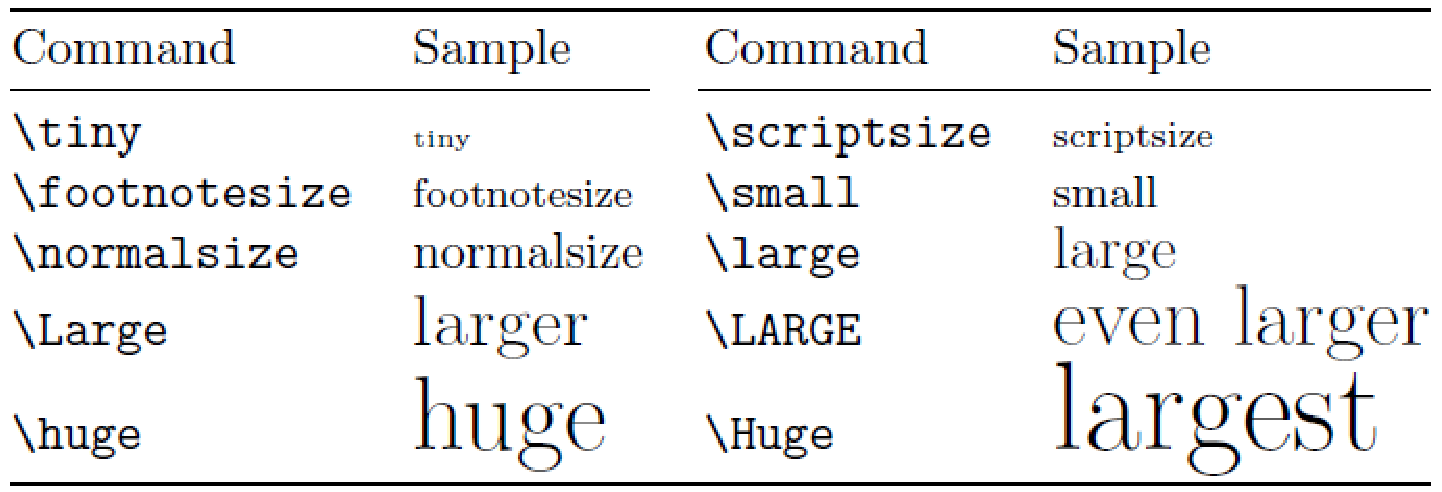
\includegraphics[width=0.7\textwidth]{img/fontsize}
% 	\caption{Exemplo de tamanhos de fonte}
% 	\label{fig:fontsize}
% \end{figure}

% \textbf{Referências dentro do Texto} Partes do texto podem ser referenciadas através do par de comandos \verb|\label| e \verb|\ref|.
%   Por exemplo, podemos inserir uma seção no artigo utilizando o seguinte comando:

% \begin{verbatim}
% \section{Seção principal}\label{sec:prcpal}
% \end{verbatim}

% Vejam que o título da seção é seguido do comando \verb|\label{nome}|.
%   Esta seção pode ser referenciada em qualquer parte do texto, como o exemplo a seguir.

% \begin{verbatim}
% Conforme explicado na Seção \ref{sec:prcpal}, nosso método utiliza...
% \end{verbatim}


% %------------------------------------------------------------------------------
% \section{Outras Dicas}
% %------------------------------------------------------------------------------

% \textbf{Caracteres Especiais} Esses não podem ser usados no texto sem a barra à frente: \# \$ \% \^{ } \& \_ \{ \} \~{ } e \slash .

% \textbf{Comentários} Comentários são precedidos de \% e podem estar em qualquer parte do texto.
%   Lembrando que tudo que estiver após \% será considerado como comentário e ignorado pelo processador.

% \textbf{Incluir Figuras} Incluir figuras no LaTeX é relativamente fácil quando se tem um formato de arquivo pré-definido.
%   or exemplo, neste documento, usa-se apenas figuras do tipo \textit{pdf}, mas também poderia-se usar do tipo \textit{png} (e \textit{jpeg}, mas este tipo não é recomendado).
%   A Tabela \ref{tab:codfig} ilustra as linhas que inserem uma figura no texto. 

% \begin{table}[!htb][ht]
%   \caption{Linhas de código para inserir figura}
% 	\centering
% 	\footnotesize	
% 		\begin{tabular}{l l}
% 	\\	\hline 
% Linha de Código & Explicação \\ \hline 
% \verb|\usepackage{graphicx}| & \textit{inclui pacote gráfico no início do documento} \\
% \verb|\begin{figure}[tb]|    & \textit{inicia figura, define sua posição no texto} \\
% \verb|\centering|            & \textit{centraliza a figura na página}\\
% \verb|\includegraphics[scale=.7]|& \textit{define escala da figura}\\
% \verb|{img/figura}|      & \textit{inclui o arquivo da figura no texto}\\
% \verb|\caption{Legenda}|     & \textit{inclui a legenda da figura}\\
% \verb|\label{fig:ap}|        & \textit{inclui o apelido da figura}\\
% \verb|\end{figure}|          & \textit{termina figura}\\
% 		\hline\end{tabular}
% 	\label{tab:codfig}
% \end{table}

% \textbf{Hifenização} Às vezes aparece uma palavra cuja hifenização, divisão silábica, está errada. Para resolver esse tipo de problema, pode-se recorrer à divisão manual da palavra, acrescentando \verb|\-| entre cada sílaba: \verb|Mi\-re\-lla|. Se, ao invés desta solução, você quiser evitar completamente que suas palavras sejam divididas, acrescente os dois comandos no início do seu documento (ou seja, antes do \\~\textit{begin\{document\}}).

% \begin{verbatim}
%   \hyphenpenalty=5000
%   \tolerance=1000
% \end{verbatim}


% \textbf{BibTeX} Para editar facilmente o BibTeX, pode-se utilizar uma ferramenta própria\footnote{Ferramentas para BibTeX: http://dmoz.org/Computers/Software/Typesetting/TeX/BibTeX}. A minha favorita é o JabRef\footnote{JabRef Editor: http://jabref.sourceforge.net/}, ilustrado na Figure \ref{fig:jabref}, porque:

% \begin{itemize}\addtolength{\itemsep}{-0.5\baselineskip}
% 	\item É de graça;
% 	\item Possui interface gráfica super intuitiva;
% 	\item Permite importar referências de bases clássicas, como ISI, Medline e RIS;
% 	\item Permite exportar para diferentes formatos, inclusive para um banco de dados utilizando SQL;
% 	\item Tem botão para procurar o artigo da respectiva referência e fazer o seu download;
% 	\item Permite adicionar comentários próprios para cada entrada;
% 	\item Pode-ser classificar as referências e criar grupos para as mesmas, e muito muito mais.
% \end{itemize}

% \begin{figure}[tb]
% 	\centering
% 		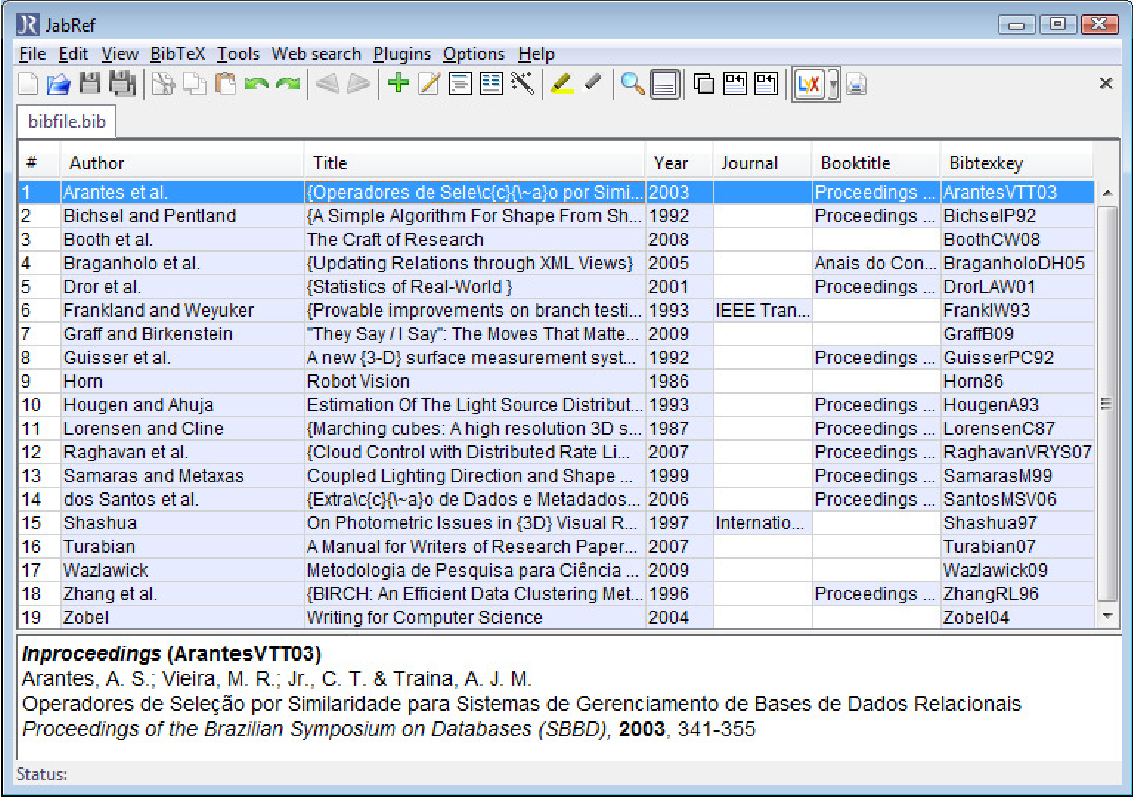
\includegraphics[width=0.98\textwidth]{img/jabref}
% 	\caption{Tela do JabRef para uma versão inicial do arquivo bib deste documento}
% 	\label{fig:jabref}
% \end{figure}

% \textbf{Listas} Listas podem ser definidas com \textit{bullets} ou com números, conforme os exemplos a seguir.

% \begin{verbatim}
% \begin{itemize}
% \item Item 1 com bullet 
% \item Item 2 com bullet 
% \end{itemize}

% \begin{enumerate}
% 	\item Item 1 numerado
% 	\item Item 2 numerado
% \end{enumerate}
% \end{verbatim}

% \textbf{Fontes Coloridas} Para adicionar texto em cores (muito útil para marcar trechos do texto que estão \textit{em trabalho}, deve-se adicionar os pacotes \textit{graphicx} e \textit{color} (usando o comando \verb|\usepackage| e depois utilizar o comando \verb|\textcolor{cor}{texto}| para colorir o \textit{texto} com a \textit{cor} especificada. Por exemplo \verb|\textcolor{blue}{texto em azul}|. Outras cores comuns são \textit{red} e \textit{green}.

% \textbf{Para Economizar Espaço} Existem alguns \textit{dirty tricks}\footnote{Ou seja, eles irão alterar a formatação dada pelo estilo default do texto.} pra economizar espaço, como por exemplo:

% -- \verb|\usepackage{times}| Usa fonte \textit{Times} no lugar da default.

% -- \verb|\usepackage[small,compact]{titlesec}| Modifica o título e os espaços antes/depois dos mesmos.

% -- \verb|\usepackage[small,it]{caption}| Reduz o tamanho das legendas de tabelas e figuras.

% \textbf{WEB} A Web é repleta de páginas e documentos sobre LaTeX. Alguns exemplos incluem:

% \begin{itemize}\addtolength{\itemsep}{-0.5\baselineskip}
%   \item Favorito inglês: \url{http://en.wikibooks.org/wiki/LaTeX/}
%   \item Favorito português: \url{http://linorg.usp.br/CTAN/info/lshort/portuguese/pt-lshort.pdf}
%   \item \url{http://www.mat.ufmg.br/~regi/topicos/intlat.pdf}
%   \item \url{http://www.duke.edu/~hg9/ctex/LaTeXManual.pdf}
%   \item \url{http://minerva.ufpel.tche.br/~campani/cursolatex.pdf}
% 	\item \url{http://www.personal.ceu.hu/tex/words.htm}
% \end{itemize}


% \end{anexosenv}


% -----------------------------------------------
% Índice Remissivo [OPCIONAL]
% -----------------------------------------------
% Veja o pacote makeindex para mais informações
\printindex


\end{document}
